%\VignetteIndexEntry{A Guide to the agop Package}
%\VignetteKeyword{agop, aggregation, preorder, mcdm}
%\VignetteEngine{knitr::knitr}
\documentclass[11pt]{article}\usepackage[]{graphicx}\usepackage[]{color}
%% maxwidth is the original width if it is less than linewidth
%% otherwise use linewidth (to make sure the graphics do not exceed the margin)
\makeatletter
\def\maxwidth{ %
  \ifdim\Gin@nat@width>\linewidth
    \linewidth
  \else
    \Gin@nat@width
  \fi
}
\makeatother

\definecolor{fgcolor}{rgb}{0.345, 0.345, 0.345}
\newcommand{\hlnum}[1]{\textcolor[rgb]{0.686,0.059,0.569}{#1}}%
\newcommand{\hlstr}[1]{\textcolor[rgb]{0.192,0.494,0.8}{#1}}%
\newcommand{\hlcom}[1]{\textcolor[rgb]{0.678,0.584,0.686}{\textit{#1}}}%
\newcommand{\hlopt}[1]{\textcolor[rgb]{0,0,0}{#1}}%
\newcommand{\hlstd}[1]{\textcolor[rgb]{0.345,0.345,0.345}{#1}}%
\newcommand{\hlkwa}[1]{\textcolor[rgb]{0.161,0.373,0.58}{\textbf{#1}}}%
\newcommand{\hlkwb}[1]{\textcolor[rgb]{0.69,0.353,0.396}{#1}}%
\newcommand{\hlkwc}[1]{\textcolor[rgb]{0.333,0.667,0.333}{#1}}%
\newcommand{\hlkwd}[1]{\textcolor[rgb]{0.737,0.353,0.396}{\textbf{#1}}}%

\usepackage{framed}
\makeatletter
\newenvironment{kframe}{%
 \def\at@end@of@kframe{}%
 \ifinner\ifhmode%
  \def\at@end@of@kframe{\end{minipage}}%
  \begin{minipage}{\columnwidth}%
 \fi\fi%
 \def\FrameCommand##1{\hskip\@totalleftmargin \hskip-\fboxsep
 \colorbox{shadecolor}{##1}\hskip-\fboxsep
     % There is no \\@totalrightmargin, so:
     \hskip-\linewidth \hskip-\@totalleftmargin \hskip\columnwidth}%
 \MakeFramed {\advance\hsize-\width
   \@totalleftmargin\z@ \linewidth\hsize
   \@setminipage}}%
 {\par\unskip\endMakeFramed%
 \at@end@of@kframe}
\makeatother

\definecolor{shadecolor}{rgb}{.97, .97, .97}
\definecolor{messagecolor}{rgb}{0, 0, 0}
\definecolor{warningcolor}{rgb}{1, 0, 1}
\definecolor{errorcolor}{rgb}{1, 0, 0}
\newenvironment{knitrout}{}{} % an empty environment to be redefined in TeX

\usepackage{alltt}

%%%%%%%%%%%%%%%%%%%%%%%%%%%%%%%%%%%%%%%%%%%%%%%%%%%%%%%%%%%%%%%%%%%%%%
%%%%%%%%%%%%%%%%%%%%%%%%%%%%%%%%%%%%%%%%%%%%%%%%%%%%%%%%%%%%%%%%%%%%%%
%%%%%%%%%%%%%%%%%%%%%%%%%%%%%%%%%%%%%%%%%%%%%%%%%%%%%%%%%%%%%%%%%%%%%%


\usepackage[dvips,a4paper,left=2.5cm,right=2.5cm,foot=1.0cm,
   headheight=1.0cm,top=2.0cm,margin=2.5cm]{geometry}
\linespread{1.1}

\usepackage{fancyhdr}


\usepackage[T1]{fontenc}
\usepackage[utf8]{inputenc}
\usepackage[english]{babel}
\selectlanguage{english}
\usepackage{xspace}
\usepackage{lmodern}

\usepackage[x11names, rgb]{xcolor}
\usepackage{tikz}
\usetikzlibrary{arrows,patterns}

\usepackage{amsmath,amssymb,amsfonts,amsthm}
\RequirePackage{graphicx,verbatim,longtable}
\usepackage{mdwlist}
\usepackage[nottoc]{tocbibind}
\usepackage{rotating}

\newcommand{\email}[1]{\href{mailto:#1}{#1}}
\renewcommand{\emph}[1]{\textbf{\textsl{#1}}}

\newcommand{\package}[1]{\textsf{#1}\xspace}
\newcommand{\program}[1]{\textsf{#1}\xspace}
\newcommand{\os}[1]{\textsf{#1}\xspace}
\newcommand{\lang}[1]{\textsf{#1}\xspace}
\newcommand{\Cpp}{\lang{C++}}
\newcommand{\R}{\lang{R}}

\newcommand{\Rfunc}[1]{\texttt{\hlkwd{#1}}}
\newcommand{\argument}[1]{\texttt{\hlkwc{#1}}}
\newcommand{\str}[1]{\texttt{\hlstr{#1}}}
\newcommand{\key}[1]{{$\langle$\texttt{#1}$\rangle$}\xspace} % skrot klawiszowy

\setlength{\pdfpagewidth}{\paperwidth}
\setlength{\pdfpageheight}{\paperheight}

% \renewcommand{\emph}{\textit}%
\newcommand{\indicator}{\text{\bf 1}}%
\renewcommand{\Pr}{\mathrm{P}}%
% \renewcommand{\ln}{\mathrm{ln}\,}%
\newcommand{\ran}{\mathrm{ran}\,}%
\newcommand{\img}{\mathrm{img}\,}%
\newcommand{\supp}{\mathrm{supp}\,}%

\newcommand{\Identity}{\mathsf{id}}


\newcommand{\vect}[1]{{\mathbf{#1}}}
\newcommand{\func}[1]{{\mathsf{#1}}}

\newcommand{\Reals}{\mathbb{R}}
\newcommand{\RealsExt}{\bar{\mathbb{R}}}
\newcommand{\Naturals}{\mathbb{N}}
\newcommand{\Ival}{\mathbb{I}}
\newcommand{\IvalPow}[1]{\mathbb{I}^{#1}}
\newcommand{\AnyPow}{^{1,2,\dots}}
\newcommand{\IvalAnyPow}{\mathbb{I}\AnyPow}
\newcommand{\Axiom}[1]{\mathrm{(#1)}}
\newcommand{\PropertyAny}[1]{\mathcal{#1}}
\newcommand{\Property}[1]{\mathcal{P}_\mathrm{(#1)}}

\usepackage{xcolor}
\definecolor{blue2}{rgb}{0,0.2,0.7}
\definecolor{red2}{rgb}{0.4,0.1,0.1}
\usepackage{colortbl}
\definecolor{navy}{rgb}{0,0.0,0.4}
\definecolor{navy2}{rgb}{0.4,0.1,0.3}
\definecolor{red2}{rgb}{0.6,0.1,0.2}
\definecolor{green2}{rgb}{0.1,0.4,0.2}

\newtheorem{theorem}{Theorem}%[section]
\newtheorem{lemma}[theorem]{Lemma}
\newtheorem{corollary}[theorem]{Corollary}
\newtheorem{proposition}[theorem]{Proposition}

\theoremstyle{remark}
\newtheorem{remark}[theorem]{Remark}

\theoremstyle{definition}
\newtheorem{definition}[theorem]{Definition}

\newtheorem{example}{Example}

\usepackage{hyperref}

\usepackage{caption}
\captionsetup{font=small,labelfont=bf,labelsep=period,justification=centering}
\addto\captionsenglish{\renewcommand{\figurename}{Fig.}}
\addto\captionsenglish{\renewcommand{\tablename}{Tab.}}


\setlength{\topsep}{3pt} % wpływa m.in. na odstęp dla verbatim
\tolerance=500
\predisplaypenalty=0
\clubpenalty=1000
\widowpenalty=1000



\newif\ifDevelopmentVersion

\DevelopmentVersiontrue



\usepackage{makeidx}
\makeindex

%%%%%%%%%%%%%%%%%%%%%%%%%%%%%%%%%%%%%%%%%%%%%%%%%%%%%%%%%%%%%%%%%%%%%%
%%%%%%%%%%%%%%%%%%%%%%%%%%%%%%%%%%%%%%%%%%%%%%%%%%%%%%%%%%%%%%%%%%%%%%
%%%%%%%%%%%%%%%%%%%%%%%%%%%%%%%%%%%%%%%%%%%%%%%%%%%%%%%%%%%%%%%%%%%%%%


\ifDevelopmentVersion
\pagestyle{fancy}
\fancyhead[L]{}
\fancyhead[R]{}
\fancyhead[C]{\footnotesize\sf This tutorial reflects the state of the most
recent development version
of \package{agop} available on
\href{https://github.com/Rexamine/agop}{\textit{GitHub}}.\newline
If you use the ``official'' CRAN release, some of the features may be unavailable.}
\fi
\IfFileExists{upquote.sty}{\usepackage{upquote}}{}
\begin{document}


\begin{center}
{\LARGE\sf A Guide to the \package{agop} {0.2-0} Package for \R}

{\large\sf\textit{Aggregation Operators and Preordered Sets in \R}}

\bigskip
{\large Marek Gagolewski${}^{1,2}$}

${}^{1}$ Systems Research Institute, Polish Academy of Sciences

ul. Newelska 6, 01-447 Warsaw, Poland

${}^{2}$ Rexamine, Email: \texttt{gagolews@rexamine.com}

\href{http://agop.rexamine.com/}%
{http://agop.rexamine.com}

\bigskip
\today


\medskip
\textit{Any suggestions and comments are welcome!}
\end{center}





\bigskip\hrule\bigskip
\tableofcontents



% \definecolor{fgcolor}{gray}{0}
% \renewcommand{\hlnumber}[1]{\textcolor[gray]{0.2}{#1}}%
% \renewcommand{\hlfunctioncall}[1]{\textbf{#1}}%
% \renewcommand{\hlstring}[1]{\textcolor[gray]{0.2}{\textit{#1}}}%
% \renewcommand{\hlkeyword}[1]{\textbf{#1}}%
% \renewcommand{\hlargument}[1]{\textcolor[rgb]{0.2,0.2,0.2}{\textsl{#1}}}%
% \renewcommand{\hlcomment}[1]{\textcolor[gray]{0.5}{\it\textsf{#1}}}%
% \renewcommand{\hlroxygencomment}[1]{\textcolor[gray]{0.5}{\it\textsf{#1}}}%
% \renewcommand{\hlformalargs}[1]{\textcolor[rgb]{0.69,0.25,0.03}{#1}}%
% \renewcommand{\hleqformalargs}[1]{\textcolor[rgb]{0.69,0.25,0.03}{#1}}%
% \renewcommand{\hlassignement}[1]{\textcolor[gray]{0}{\textbf{#1}}}%
% \renewcommand{\hlpackage}[1]{\textcolor[rgb]{0.59,0.71,0.15}{#1}}%
% \renewcommand{\hlslot}[1]{\textit{#1}}%
% \renewcommand{\hlsymbol}[1]{\textcolor[cmyk]{0,0,0,1}{#1}}%
% \renewcommand{\hlprompt}[1]{\textcolor[cmyk]{0,0,0,0.5}{#1}}%

%%%%%%%%%%%%%%%%%%%%%%%%%%%%%%%%%%%%%%%%%%%%%%%%%%%%%%%%%%%%%%%%%%%%%
%%%%%%%%%%%%%%%%%%%%%%%%%%%%%%%%%%%%%%%%%%%%%%%%%%%%%%%%%%%%%%%%%%%%%
%%%%%%%%%%%%%%%%%%%%%%%%%%%%%%%%%%%%%%%%%%%%%%%%%%%%%%%%%%%%%%%%%%%%%




\section{Getting Started}

\begin{quotation}\it\noindent
``The process of combining several numerical values into a single
representative one is called \textbf{aggregation}, and the numerical function
performing this process is called \textbf{aggregation function}.
This simple definition
demonstrates the size of the field of application of aggregation:
applied mathematics
(e.g.~probability, statistics, decision theory), computer science
(e.g.~artificial
intelligence, operation research), as well as many applied fields
(economics and finance,
pattern recognition and image processing, data fusion,
multicriteria decision making,
automated reasoning etc.). Although history of aggregation is probably
as old as mathematics (think of the arithmetic mean), its existence
has reminded underground till only recent (\dots).''
\cite[p.~xiii]{GrabischETAL2009:aggregationfunctions}
\end{quotation}


\bigskip
\R \cite{Rproject:home} is a free, open source software environment
for statistical computing and graphics, which
includes an implementation
of a very powerful and quite popular high-level language called~\lang{S}.
It runs on all major operating systems, i.e.~\os{Windows},
\os{Linux}, and \os{MacOS X}.
To install \R and/or find some information on the \lang{S} language
please visit \R Project's Homepage at \href{http://www.R-project.org}{www.R-project.org}.
Perhaps you may also wish to install  \program{RStudio},
a convenient development environment for \R.
It is available at \href{http://rstudio.org/}{www.rsudio.org}.


\bigskip
\package{agop} is an open source (licensed under GNU LGPL 3)
package for \R$\ge$ 2.12 to which anyone can contribute.
It started as a fork of the \package{CITAN} (\textit{Citation
Analysis Toolpack}, \cite{Gagolewski2011:CITAN}) package.

To install latest ``official'' release of the
package available on \textit{CRAN} we type%
\ifDevelopmentVersion%
\footnote{You are viewing the \textbf{development} version of the tutorial.
Some of the features presented in this document may be missing
in the CRAN release. Please, upgrade to the \textbf{latest} development version from
\href{https://github.com/Rexamine/agop}{\textit{GitHub}}
if you need the new functionality.
Note that you will need a working \lang{C}/\lang{C++} compiler.}\ignorespaces
\fi%
:

\begin{knitrout}\small
\definecolor{shadecolor}{rgb}{0.969, 0.969, 0.969}\color{fgcolor}\begin{kframe}
\begin{alltt}
\hlkwd{install.packages}\hlstd{(}\hlstr{'agop'}\hlstd{)}
\end{alltt}
\end{kframe}
\end{knitrout}

\noindent
Alternatively, we may fetch its current development snapshot
from \href{https://github.com/Rexamine/agop}{\textit{GitHub}}:

\begin{knitrout}\small
\definecolor{shadecolor}{rgb}{0.969, 0.969, 0.969}\color{fgcolor}\begin{kframe}
\begin{alltt}
\hlkwd{install.packages}\hlstd{(}\hlstr{'devtools'}\hlstd{)}
\hlstd{devtools::}\hlkwd{install_github}\hlstd{(}\hlstr{'agop'}\hlstd{,} \hlstr{'Rexamine'}\hlstd{)}
\end{alltt}
\end{kframe}
\end{knitrout}

\noindent
Note that in this case you will need a working \lang{C}/\lang{C++} compiler%
\footnote{\os{Windows} users should have \textsf{Rtools} installed,
see \href{http://cran.r-project.org/bin/windows/Rtools/}%
{cran.r-project.org/bin/windows/Rtools/}.}.


\bigskip
Each session with \package{agop} should be preceded by
a call to:

\begin{knitrout}\small
\definecolor{shadecolor}{rgb}{0.969, 0.969, 0.969}\color{fgcolor}\begin{kframe}
\begin{alltt}
\hlkwd{library}\hlstd{(}\hlstr{'agop'}\hlstd{)} \hlcom{# Load the package}
\end{alltt}
\end{kframe}
\end{knitrout}

\bigskip
To view the main page of the manual we type:

\begin{knitrout}\small
\definecolor{shadecolor}{rgb}{0.969, 0.969, 0.969}\color{fgcolor}\begin{kframe}
\begin{alltt}
\hlkwd{library}\hlstd{(}\hlkwc{help}\hlstd{=}\hlstr{'agop'}\hlstd{)}
\end{alltt}
\end{kframe}
\end{knitrout}

\noindent
For more information please visit the package's homepage \cite{GagolewskiCena:agoppackage}.
In case of any problems, comments, or suggestions feel free to contact the authors.
Good luck!



%%%%%%%%%%%%%%%%%%%%%%%%%%%%%%%%%%%%%%%%%%%%%%%%%%%%%%%%%%%%%%%%%%%%%
%%%%%%%%%%%%%%%%%%%%%%%%%%%%%%%%%%%%%%%%%%%%%%%%%%%%%%%%%%%%%%%%%%%%%
%%%%%%%%%%%%%%%%%%%%%%%%%%%%%%%%%%%%%%%%%%%%%%%%%%%%%%%%%%%%%%%%%%%%%




\section{Theoretical Background}

Let us establish some basic notation convention
used throughout this tutorial.
From now on let $\Ival=[a,b]$, possibly with $a=-\infty$ or $b=\infty$.
Note that in many practical situations we commonly choose $\Ival=[-1,1]$,
$\Ival=[0,1]$ or $\Ival=[0,\infty]$.
A set of all vectors of arbitrary length  with elements in $\Ival$
is denoted by $\IvalAnyPow=\bigcup_{n=1}^\infty \IvalPow{n}$ .

For two equal-length vectors $\vect{x}, \vect{y}\in\IvalPow{n}$
we write $\vect{x}\le_n\vect{y}$ if and only
if for all $i=1,\dots,n$ it holds $x_i\le y_i$.
Moreover, all binary arithmetic operations on vectors
$\vect{x}, \vect{y}\in\IvalPow{n}$ will be performed element-wise,
e.g. $\vect{x}+\vect{y}=(x_1+y_1,\dots,x_n+y_n)\in\IvalPow{n}$.
Similar behavior is assumed for
$-$, $\cdot$, $/$, $\wedge$ (min), $\vee$ (max), etc.
Additionally, each function of one variable
$\func{f}:\Ival\to\Ival$ can be extended to the vector
space: we write $\func{f}(\vect{x})$ to denote
$(\func{f}(x_1), \dots, \func{f}(x_n))$.


Let $x_{(i)}$ denote the $i$th order statistic,
i.e.~the $i$th smallest value in $\vect{x}$.
Moreover, for convenience,
let $x_{\{i\}}=x_{|\vect{x}|-i+1}$ denote the $i$th greatest value in $\vect{x}$.

For any $n\in\mathbb{N}$ and $c\in\Ival$,
we set $(n\ast c) = (c,\dots,c)\in\IvalPow{n}$.
Also, $[n]:=\{1,2,\dots,n\}$ with $[0]=\emptyset$.

Let $\mathfrak{S}_{[n]}$ denote the set of all permutations of $[n]$,
and for any $\sigma\in\mathfrak{S}_{[n]}$, $\IvalPow{n}_\sigma=\{(x_1,\dots,x_n)\in\IvalPow{n}:
x_{\sigma(1)}\le\dots\le x_{\sigma(n)}\}$.
Furthermore, if $\func{F}:\IvalPow{n}\to\Ival$,
then let $\func{F}|_\sigma$ denote the restriction
of $\func{F}$ to $\IvalPow{n}_\sigma$, i.e.~$\func{F}|_\sigma:\IvalPow{n}_\sigma\to\Ival$,
$\func{F}|_\sigma(\vect{x})=\func{F}(\vect{x})$ for any $\vect{x}\in\IvalPow{n}_\sigma$.


\subsection{A Note on Representing Numeric Data and Applying Operations in \R}

Recall how we create numeric vectors in \R:

\begin{knitrout}\small
\definecolor{shadecolor}{rgb}{0.969, 0.969, 0.969}\color{fgcolor}\begin{kframe}
\begin{alltt}
\hlstd{(x1} \hlkwb{<-} \hlkwd{c}\hlstd{(}\hlnum{5}\hlstd{,} \hlnum{2}\hlstd{,} \hlnum{3}\hlstd{,} \hlnum{1}\hlstd{,} \hlnum{0}\hlstd{,} \hlnum{0}\hlstd{))}
\end{alltt}
\begin{verbatim}
## [1] 5 2 3 1 0 0
\end{verbatim}
\begin{alltt}
\hlkwd{class}\hlstd{(x1)}
\end{alltt}
\begin{verbatim}
## [1] "numeric"
\end{verbatim}
\begin{alltt}
\hlstd{(x2} \hlkwb{<-} \hlnum{10}\hlopt{:}\hlnum{1}\hlstd{)} \hlcom{# the same as seq(10, 1)}
\end{alltt}
\begin{verbatim}
##  [1] 10  9  8  7  6  5  4  3  2  1
\end{verbatim}
\begin{alltt}
\hlstd{(x3} \hlkwb{<-} \hlkwd{seq}\hlstd{(}\hlnum{1}\hlstd{,} \hlnum{5}\hlstd{,} \hlkwc{length.out}\hlstd{=}\hlnum{6}\hlstd{))}
\end{alltt}
\begin{verbatim}
## [1] 1.0 1.8 2.6 3.4 4.2 5.0
\end{verbatim}
\begin{alltt}
\hlstd{(x4} \hlkwb{<-} \hlkwd{seq}\hlstd{(}\hlnum{1}\hlstd{,} \hlnum{5}\hlstd{,} \hlkwc{by}\hlstd{=}\hlnum{1.25}\hlstd{))}
\end{alltt}
\begin{verbatim}
## [1] 1.00 2.25 3.50 4.75
\end{verbatim}
\end{kframe}
\end{knitrout}

To obtain $(n\ast c)$, e.g.~for $n=10$ and $c=3$, we call:

\begin{knitrout}\small
\definecolor{shadecolor}{rgb}{0.969, 0.969, 0.969}\color{fgcolor}\begin{kframe}
\begin{alltt}
\hlkwd{rep}\hlstd{(}\hlnum{10}\hlstd{,} \hlnum{3}\hlstd{)}
\end{alltt}
\begin{verbatim}
## [1] 10 10 10
\end{verbatim}
\end{kframe}
\end{knitrout}

Note that in \R{} all the arithmetic operations on vectors are
performed element-wise, i.e.~in a manner indicated above.
This is called \emph{vectorization}.
The same holds for mathematical functions: they are extended to the vector space.

\begin{knitrout}\small
\definecolor{shadecolor}{rgb}{0.969, 0.969, 0.969}\color{fgcolor}\begin{kframe}
\begin{alltt}
\hlstd{x} \hlkwb{<-} \hlkwd{c}\hlstd{(}\hlnum{1}\hlstd{,} \hlnum{3}\hlstd{,}  \hlnum{3}\hlstd{,} \hlnum{2}\hlstd{)}
\hlstd{y} \hlkwb{<-} \hlkwd{c}\hlstd{(}\hlnum{2}\hlstd{,} \hlnum{3}\hlstd{,} \hlopt{-}\hlnum{1}\hlstd{,} \hlnum{0}\hlstd{)}
\hlstd{x}\hlopt{+}\hlstd{y}
\end{alltt}
\begin{verbatim}
## [1] 3 6 2 2
\end{verbatim}
\begin{alltt}
\hlstd{x}\hlopt{*}\hlstd{y}
\end{alltt}
\begin{verbatim}
## [1]  2  9 -3  0
\end{verbatim}
\begin{alltt}
\hlkwd{pmin}\hlstd{(x,y)} \hlcom{# parallel minimum}
\end{alltt}
\begin{verbatim}
## [1]  1  3 -1  0
\end{verbatim}
\begin{alltt}
\hlkwd{pmax}\hlstd{(x,y)} \hlcom{# parallel maximum}
\end{alltt}
\begin{verbatim}
## [1] 2 3 3 2
\end{verbatim}
\begin{alltt}
\hlkwd{abs}\hlstd{(y)}
\end{alltt}
\begin{verbatim}
## [1] 2 3 1 0
\end{verbatim}
\end{kframe}
\end{knitrout}

\noindent
Thus, we calculated $\vect{x}+\vect{y}$,
$\vect{x}\cdot\vect{y}$, $\vect{x}\wedge\vect{y}$, $\vect{x}\vee\vect{y}$,
and $|\vect{x}|$
(try to determine yourself what happens if we deal
with two vectors of unequal length in \R).

Moreover, given two equal-length vectors,
for the $\le_n$ relation we write:

\begin{knitrout}\small
\definecolor{shadecolor}{rgb}{0.969, 0.969, 0.969}\color{fgcolor}\begin{kframe}
\begin{alltt}
\hlkwd{all}\hlstd{(x} \hlopt{<=} \hlstd{y)}
\end{alltt}
\begin{verbatim}
## [1] FALSE
\end{verbatim}
\end{kframe}
\end{knitrout}

To get $x_{\{i\}}$ we have to sort the given vector nonincreasingly:

\begin{knitrout}\small
\definecolor{shadecolor}{rgb}{0.969, 0.969, 0.969}\color{fgcolor}\begin{kframe}
\begin{alltt}
\hlstd{(xg} \hlkwb{<-} \hlkwd{sort}\hlstd{(x,} \hlkwc{decreasing}\hlstd{=}\hlnum{TRUE}\hlstd{))} \hlcom{# `decresing' may be misleading}
\end{alltt}
\begin{verbatim}
## [1] 3 3 2 1
\end{verbatim}
\begin{alltt}
\hlstd{xg[}\hlnum{3}\hlstd{]} \hlcom{# the third greatest value in x}
\end{alltt}
\begin{verbatim}
## [1] 2
\end{verbatim}
\end{kframe}
\end{knitrout}

\noindent
and for $x_{(i)}$ we type:

\begin{knitrout}\small
\definecolor{shadecolor}{rgb}{0.969, 0.969, 0.969}\color{fgcolor}\begin{kframe}
\begin{alltt}
\hlstd{(xs} \hlkwb{<-} \hlkwd{sort}\hlstd{(x))} \hlcom{# sorted nondecreasingly}
\end{alltt}
\begin{verbatim}
## [1] 1 2 3 3
\end{verbatim}
\begin{alltt}
\hlstd{xs[}\hlnum{3}\hlstd{]} \hlcom{# the third smallest value in x}
\end{alltt}
\begin{verbatim}
## [1] 3
\end{verbatim}
\end{kframe}
\end{knitrout}


\subsection{A Note on Storing Multiple Numeric Vectors in \R}

Vectors of the same length can be conveniently stored in a matrices.
Keep in mind that elements are stored in a columnwise order,
so for performance reasons please do store each vector in
a separate matrix's column (not: row).
Please note
that the \argument{dimnames} attribute of a matrix may define
its row and column labels.
Its value may be set to \texttt{NULL}
(no names given) or to a list with two character
vectors (rows and columns names, respectively).
Another simple way to set the labels is by using
the \Rfunc{rownames()} and \Rfunc{colnames()} functions.

The \Rfunc{apply()} function may be called to evaluate
a given method on each matrix row  or column
(parameter \argument{MARGIN} set to 1 and 2, respectively).


\begin{knitrout}\small
\definecolor{shadecolor}{rgb}{0.969, 0.969, 0.969}\color{fgcolor}\begin{kframe}
\begin{alltt}
\hlstd{expertopinions} \hlkwb{<-} \hlkwd{matrix}\hlstd{(}\hlkwd{c}\hlstd{(}
      \hlnum{6}\hlstd{,}\hlnum{7}\hlstd{,}\hlnum{2}\hlstd{,}\hlnum{3}\hlstd{,}\hlnum{1}\hlstd{,} \hlcom{# this will be the first COLUMN}
      \hlnum{8}\hlstd{,}\hlnum{3}\hlstd{,}\hlnum{2}\hlstd{,}\hlnum{1}\hlstd{,}\hlnum{9}\hlstd{,} \hlcom{# 2nd}
      \hlnum{4}\hlstd{,}\hlnum{2}\hlstd{,}\hlnum{4}\hlstd{,}\hlnum{1}\hlstd{,}\hlnum{6}  \hlcom{# 3rd}
   \hlstd{),}
   \hlkwc{ncol}\hlstd{=}\hlnum{3}\hlstd{,}
   \hlkwc{dimnames}\hlstd{=}\hlkwd{list}\hlstd{(}\hlkwa{NULL}\hlstd{,} \hlkwd{c}\hlstd{(}\hlstr{"A"}\hlstd{,} \hlstr{"B"}\hlstd{,} \hlstr{"C"}\hlstd{))} \hlcom{# only column names set}
\hlstd{)}
\hlkwd{class}\hlstd{(expertopinions)}
\end{alltt}
\begin{verbatim}
## [1] "matrix"
\end{verbatim}
\begin{alltt}
\hlkwd{print}\hlstd{(expertopinions)}   \hlcom{# or print(authors)}
\end{alltt}
\begin{verbatim}
##      A B C
## [1,] 6 8 4
## [2,] 7 3 2
## [3,] 2 2 4
## [4,] 3 1 1
## [5,] 1 9 6
\end{verbatim}
\begin{alltt}
\hlkwd{apply}\hlstd{(expertopinions,} \hlnum{2}\hlstd{, mean)} \hlcom{#  apply the mean() function on each COLUMN}
\end{alltt}
\begin{verbatim}
##   A   B   C 
## 3.8 4.6 3.4
\end{verbatim}
\end{kframe}
\end{knitrout}

Vectors that are not of the same length may be store in a list (with
possibly named elements). In that case, the functionality
of \Rfunc{apply()} is provided by \Rfunc{lapply()} or
\Rfunc{sapply()} functions.

\begin{knitrout}\small
\definecolor{shadecolor}{rgb}{0.969, 0.969, 0.969}\color{fgcolor}\begin{kframe}
\begin{alltt}
\hlstd{authors} \hlkwb{<-} \hlkwd{list}\hlstd{(}
   \hlstr{"John S."} \hlstd{=} \hlkwd{c}\hlstd{(}\hlnum{7}\hlstd{,}\hlnum{6}\hlstd{,}\hlnum{2}\hlstd{,}\hlnum{1}\hlstd{,}\hlnum{0}\hlstd{),}
   \hlstr{"Kate F."} \hlstd{=} \hlkwd{c}\hlstd{(}\hlnum{9}\hlstd{,}\hlnum{8}\hlstd{,}\hlnum{7}\hlstd{,}\hlnum{6}\hlstd{,}\hlnum{4}\hlstd{,}\hlnum{1}\hlstd{,}\hlnum{1}\hlstd{,}\hlnum{0}\hlstd{)}
\hlstd{)}
\hlkwd{class}\hlstd{(authors)}
\end{alltt}
\begin{verbatim}
## [1] "list"
\end{verbatim}
\begin{alltt}
\hlkwd{str}\hlstd{(authors)}   \hlcom{# or print(authors)}
\end{alltt}
\begin{verbatim}
## List of 2
##  $ John S.: num [1:5] 7 6 2 1 0
##  $ Kate F.: num [1:8] 9 8 7 6 4 1 1 0
\end{verbatim}
\begin{alltt}
\hlkwd{index_h}\hlstd{(authors[[}\hlnum{1}\hlstd{]])} \hlcom{# the h-index /see below/ for 1st author}
\end{alltt}
\begin{verbatim}
## [1] 2
\end{verbatim}
\begin{alltt}
\hlkwd{sapply}\hlstd{(authors, index_h)} \hlcom{# calculate the h-index for all vectors in a list}
\end{alltt}
\begin{verbatim}
## John S. Kate F. 
##       2       4
\end{verbatim}
\end{kframe}
\end{knitrout}





\subsection{Aggregation Operators and Their Basic Properties}

Dealing with huge amounts of data
faces us with the problem of constructing their synthetic descriptions.
The aggregation theory,
a relatively new research domain at the border of mathematics and
computer science, is interested in the analysis
of functions that may be used in this task.
Thus, we should start with the formal definition of
objects of our interest.
Here is the most general setting:


% Aggregation theory finds its applications in all the fields,
% where aggregating information is important: applied and pure mathematics,
% e.g. probability, statistics, decision theory, functional equations, operation
% research, computer sciences, social science, economics and finance,
% pattern recognition and so on.
%
% In its simplest definition aggregation denote process of
% combining several numerical values into one, representative for the whole input.

\begin{definition}
A function $\func{F}: \IvalAnyPow\to\Ival$
is called an \emph{(extended\footnote{Extended to the
space of vectors of arbitrary length, cf.~e.g.~\cite{CalvoMayor1999:remarks2eaf,
GrabischETAL2009:aggregationfunctions}; Classical approach
considers only fixed-length vectors.
In \package{agop} we are as much general as possible.}) aggregation operator}
if it is at least \emph{nondecreasing} in each variable,
i.e.~for all $n$ and $\vect{x},\vect{y}\in\IvalPow{n}$
if $\vect{x}\le_n\vect{y}$, then $\func{F}(\vect{x})\le\func{F}(\vect{y})$.
\end{definition}

Note that each aggregation operator is a mapping into $\Ival$,
thus for all $n$ we have $\inf_{\vect{x}\in\IvalPow{n}} \func{F}(\vect{x}) \ge a$
and $\sup_{\vect{x}\in\IvalPow{n}} \func{F}(\vect{x}) \le b$.
By nondecreasingness, however, these conditions reduce to
$\func{F}(n\ast a)\ge a$ and $\func{F}(n\ast b)\le b$.

Also keep in mind that some authors assume
(cf.~\cite{GrabischETAL2009:aggregationfunctions})\label{Prop:StrongBoundaryCond}
that aggregation operators must fulfill the two following \emph{strong boundary
conditions}: for all $n$ we have
$\inf_{\vect{x}\in\IvalPow{n}} \func{F}(\vect{x}) =a$
and $\sup_{\vect{x}\in\IvalPow{n}} \func{F}(\vect{x})= b$.
Such aggregation operators are sometimes called \emph{averaging functions}.
In our case, this does not necessarily hold -- we want to be
more general.


\bigskip
Here are some interesting properties of averaging functions.
Later on we will characterize some of the classes of functions
that fulfill them.

\begin{definition}
We call $\func{F}: \IvalAnyPow\to\Ival$ \emph{symmetric} if:
\[
(\forall n\in\mathbb{N})\ (\forall \vect{x},\vect{y}\in\IvalPow{n})\
\vect{x}\cong\vect{y}\Longrightarrow\func{F}(\vect{x})=\func{F}(\vect{y}),
 \]
 where  $\vect{x}\cong\vect{y}$ if and only if there exists a permutation
$\sigma$ of $[n]$ such that
$\vect{x}=(y_{\sigma(1)},\dots,y_{\sigma(n)})$.
\end{definition}

It may be shown, see
\cite[Thm.~2.34]{GrabischETAL2009:aggregationfunctions}, that
$\func{F}:\IvalPow{n}\to\Ival$ is symmetric if and only if there exists
a function $\func{G}':\IvalAnyPow\to\Ival$ such that
$\func{F}(x_{1},\dots,x_{n})=\func{G}'(x_{(1)},\dots,x_{(n)})$,
or, equivalently, a function $\func{G}'':\IvalAnyPow\to\Ival$,
for which we have
$\func{F}(x_{1},\dots,x_{n})=\func{G}''(x_{\{1\}},\dots,x_{\{n\}})$.
In other words, $\func{F}$
may be defined solely using order statistics:
its value is independent
of the aggregated vector's elements presentation.


By the way:

\begin{knitrout}\small
\definecolor{shadecolor}{rgb}{0.969, 0.969, 0.969}\color{fgcolor}\begin{kframe}
\begin{alltt}
\hlstd{x} \hlkwb{<-} \hlkwd{c}\hlstd{(}\hlnum{0.5}\hlstd{,} \hlnum{0.4}\hlstd{,} \hlnum{0.1}\hlstd{,} \hlnum{0.3}\hlstd{,} \hlnum{0.2}\hlstd{)} \hlcom{# an exemplary vector}
\hlstd{sigma1} \hlkwb{<-} \hlkwd{c}\hlstd{(}\hlnum{1}\hlstd{,} \hlnum{3}\hlstd{,} \hlnum{5}\hlstd{,} \hlnum{2}\hlstd{,} \hlnum{4}\hlstd{)} \hlcom{# an exemplary permutation}
\hlstd{x[sigma1]}
\end{alltt}
\begin{verbatim}
## [1] 0.5 0.1 0.2 0.4 0.3
\end{verbatim}
\begin{alltt}
\hlstd{(sigma2} \hlkwb{<-} \hlkwd{order}\hlstd{(x))} \hlcom{# ordering permutation of x}
\end{alltt}
\begin{verbatim}
## [1] 3 5 4 2 1
\end{verbatim}
\begin{alltt}
\hlstd{x[sigma2]}
\end{alltt}
\begin{verbatim}
## [1] 0.1 0.2 0.3 0.4 0.5
\end{verbatim}
\end{kframe}
\end{knitrout}

\medskip
Idempotence is well-known from algebra,
where we say that element $x$ is idempotent with respect
to binary operator $*$ if we have $x*x=x$. The following definition
extends this property to $n$-ary aggregation functions,
cf.~\cite{GrabischETAL2009:aggregationfunctions}.
% to bym sobie darowal - latwo zauwazyc:
% for which it simply means that
% for $\vect{x}\in\IvalPow{n}$ such that $x_{i}=x$ for all $i=1,\dots,n$, we have
% $\func{F}(\vect{x})=x$.

\begin{definition}
We call $\func{F}: \IvalAnyPow\to\Ival$ \emph{idempotent} if:
\[(\forall n\in\mathbb{N})\ (\forall x\in\Ival)\ \func{F}(n\ast x)=x.\]
\end{definition}

Idempotent aggregation operators fulfilling
the strong boundary conditions (see p.~\pageref{Prop:StrongBoundaryCond})
are sometimes called \emph{averaging functions}, cf.~\cite{GrabischETAL2009:aggregationfunctions}.
%%%%%%%%%%%%%%%%znalezc prace

An example of such object is the arithmetic mean or median.

\medskip
\begin{definition}
We call $\func{F}: \IvalAnyPow\to\Ival$ \emph{additive} if:
\[
\func{F}(\vect{x}+\vect{y})=\func{F}(\vect{x})+\func{F}(\vect{y}),
\]
for all $n\in\mathbb{N}, \vect{x}, \vect{y}\in\IvalPow{n}$ such that
$\vect{x}+\vect{y}\in\IvalPow{n}$.
\end{definition}
Please note that for $a\leq 0$, if $\func{F}$ is additive,
then necessarily it holds $\func{F}(\vect{0})=0$.

\medskip
\begin{definition}
We call $\func{F}$ \emph{minitive} if:
\[
(\forall n\in\mathbb{N})\ (\forall \vect{x},\vect{y}\in\IvalPow{n})\
\func{F}(\vect{x}\wedge
\vect{y})=\func{F}(\vect{x})\wedge\func{F}(\vect{y}).
\]
\end{definition}

\medskip
\begin{definition}
We call $\func{F}$ \emph{maxitive} if:
\[
(\forall n\in\mathbb{N})\ (\forall \vect{x},\vect{y}\in\IvalPow{n})\
\func{F}(\vect{x}\vee
\vect{y})=\func{F}(\vect{x})\vee\func{F}(\vect{y}).
\]
\end{definition}

\medskip
%%%%%%% podaje trzy: Beliakov, Grabish i Mesiar-Mesiarowa

\begin{definition}
We call $\func{F}$ \emph{modular}
(cf.~\cite{BeliakovETAL2007:aggregationpractitioners,
GrabischETAL2009:aggregationfunctions,
MesiarMesiarova2011:OMA}) if:
\[
(\forall n\in\mathbb{N})\ (\forall \vect{x},\vect{y}\in\IvalPow{n})\
\func{F}(\vect{x}\vee\vect{y})
+\func{F}(\vect{x}\wedge\vect{y})=\func{F}(\vect{x})+\func{F}
(\vect{y})
\]
%
\end{definition}

It may easily be seen that each additive operator
%fulfiling the lower strong boundary condition
is also modular
(i.e.~modularity is more general than additivity),
because for any additive aggregation operator $\func{F}$,
since
$(\vect{x}\vee\vect{y})+(\vect{x}\wedge\vect{y})=\vect{x}+\vect{y}$,
we have $\func{F}(\vect{x})+\func{F}(\vect{y})=\func{F}(\vect{x}+\vect{y})=
\func{F}((\vect{x}\vee\vect{y})+(\vect{x}\wedge\vect{y}))
=\func{F}(\vect{x}\vee\vect{y})+\func{F}(\vect{x}\wedge\vect{y})$.


\medskip
Apart from the ``ordinary'' minitivity, maxitivity, and modularity
we may introduce their symmetrized versions,
using $\vect{x}\stackrel{S}{+}\vect{y}
=(x_{(1)}+ y_{(1)},\dots,x_{(n)}+y_{(n)})$,
$\vect{x}\stackrel{S}{\vee}\vect{y}
=(x_{(1)}\vee y_{(1)},\dots,x_{(n)}\vee   y_{(n)})$
and
$\vect{x}\stackrel{S}{\wedge}\vect{y}
=(x_{(1)}\wedge y_{(1)},\dots,x_{(n)}\wedge y_{(n)})$.


\subsection{Impact Functions and The Producers Assessment Problem}

We already noticed the important class of aggregation operators:
the averaging functions. They may be used to represent the most ``typical''
value of a numeric vector.
Here is another interesting class
that represents solutions to some very interesting practical issue.

The \emph{Producers Assessment Problem} (PAP,
\cite{GagolewskiGrzegorzewski2011:ijar}) concerns evaluation of a set of
\emph{producers} (e.g.~scientists, artists, writers, craftsman)
according to some quality or popularity \emph{ratings}
% (e.g.~the number of articles'
% citations, the number of sold book copies etc.)
of \emph{products}
(e.g.~scientific articles, works, books, artifacts) that
were outputted by an entity.


\begin{table}[ht]
\centering
\caption{\label{Table:InstancesPAP} The Producer
Assessment Problem -- typical instances}

\noindent\footnotesize
\begin{tabular}{|c||llp{3.5cm}p{3.2cm}|}
\hline
& Producer & Products & Rating method & Discipline \\
\hline\hline
A & Scientist & Scientific articles & Number of citations & Scientometrics \\
\hline
B & Scientific institute & Scientists & The $h$-index & Scientometrics     \\
\hline
C & Web server & Web pages & Number of in-links & Webometrics   \\
\hline
D & Artist   & Paintings  & Auction price & Auctions \\
\hline
E & Billboard company & Advertisements & Sale results & Marketing \\
\hline
F & \R{} package author & Packages & PageRank values w.r.t.~the dependency graph & Software Engineering\\
% \dots & \dots & \dots & \dots \\
\hline
\end{tabular}
\end{table}

PAP instances may be found in many real-life
situations, like those encountered
for example in scientometrics, webometrics, marketing,
manufacturing, or quality
engineering, see Table~\ref{Table:InstancesPAP}
and e.g.~\cite{FranceschiniMaisano2009:hmanufacturing}.
Our main interest here is focused on constructing and analyzing
aggregation operators which may be used in the producers' rating task.
Such functions should take into account the two following
aspects of a producer's quality:
\begin{itemize}
\item his/her ability to output highly-rated products,
\item his/her overall productivity.
\end{itemize}

For the sake of illustration, we will consider PAP in the
scientometric context, where scientists ``produce''
papers that are cited by peers.

Let $\Ival=[0,\infty]$ represent the set of values that some a~priori chosen
paper quality measure may take. These may of course be non-integers,
for example when we consider citations normalized with respect
to the number of papers' authors.


It is widely accepted, see e.g.~\cite{Woeginger2008:axiomatich,
Woeginger2008:axiomaticg,
Woeginger2008:symmetryaxiom,Rousseau2008:woegingerax,Quesada2009:monotonicityh,
Quesada2010:moreaxiomatics,GagolewskiGrzegorzewski2011:ijar,
Gagolewski2011:PhD,FranceschiniMaisano2011:structevalh},
that each aggregation operator
 $\func{F}:\IvalAnyPow\to\Ival$ to be applied in  PAP  should at least be:
\begin{enumerate}
   \item[(a)] nondecreasing in each variable (additional
   citations received by a paper or an improvement
   of its quality measure does not result
   in a decrease of the authors' overall evaluation),
   \item[(b)] arity-monotonic (by publishing a new paper we
   never decrease the overall valuation of the entity),
   \item[(c)] symmetric (independent
of the order of elements' presentation, i.e.~we may always assume that
we aggregate vectors that are already sorted).
\end{enumerate}
% Conditions (a) and (b) imply that each impact function
% is able -- at least potentially -- to describe two ``dimensions''
% of the author's output quality: (a) his/her ability to write
% eagerly-cited or highly-valuated papers and (b) his/her overall productivity.

% More formally, condition (a) holds if and only if for each
% $n$ and $\vect{x},\vect{y}\in\IvalPow{n}$ such that $(\forall i)$
% $x_i\le y_i$ we have $\func{J}(\vect{x})\le\func{J}(\vect{y})$.
% On the other hand,
More formally, axiom (b) is fulfilled iff
for any $\vect{x}\in\IvalAnyPow$ and $y\in\Ival$ it holds
$\func{F}(\vect{x})\le\func{F}(x_1,\dots,x_n,y)$.
It may be seen that this property is \emph{arity-dependent},
i.e.~it takes into account the number of elements to be aggregated.

Moreover, (a) and (c) were defined in the previous section.
% Lastly, requirement (c) holds iff for all $n$ and $\vect{x}\in\IvalPow{n}$
% we have $\func{J}(\vect{x})=\func{J}(x_{\{1\}},\dots,x_{\{n\}})$,
% where $x_{\{i\}}$ denotes the $i$th largest value from $\vect{x}$,
% i.e.~its $(n-i+1)$th order statistic.

\bigskip
Here is a bunch of arity-dependent properties
that can  be useful while aggregating vectors
of varying lengths, cf.~also \cite{CenaGagolewski2014:om3fss}.
% This model described situation when a~``producer'' whose quality
% has to be assessed ``outputs'' yet another ``product'' and we have to reevaluate
% his/her rating.


\begin{definition}\label{Def:zero_insensitive}
We call $\func{F}\in \mathcal{E}(\Ival)$ a
\emph{zero-insensitive} aggregation operator if
for each $\vect{x}\in\IvalAnyPow$ it holds
\(
\func{F}(\vect{x},0)=\func{F}(\vect{x}).
\)
\end{definition}

% In other words, if $\func{F}$ is zero-insensitive, then $0$ is its
% so-called extended neutral element, see
% \cite[Def.~2.108]{GrabischETAL2009:aggregationfunctions}.
% What is more, $0$ is an idempotent element of every zero-insensitive function
% $\func{F}$
% such that $\func{F}(0)=0$.

It may be seen that, under nondecreasingness,
zero-insensitivity implies arity-monotonicity,
see \cite{GagolewskiGrzegorzewski2010:ipmu}.
What is interesting, each zero-insensitive impact function $\func{F}$
may be defined by means of $\func{G}:\IvalPow{\infty}\to\Ival$
such that $\func{F}(\vect{x}) = \func{G}(\vect{x},0,0,\dots)$,
i.e.~of function which domain is the space of vectors of infinite length.

Zero-sensitivity may be strengthened as follows,
cf.~\cite{GagolewskiGrzegorzewski2010:ipmu}
and \cite[Axiom A1]{Woeginger2008:axiomatich}.


\begin{definition}\label{Def:Wlasnosc_F-}
$\func{F}\in \mathcal{E}(\Ival)$ is \emph{$F$-insensitive} if
\begin{equation*}
(\forall \vect{x}\in\IvalAnyPow)\ (\forall y\in\Ival)\ y\le\func{F}(\vect{x})
\Longrightarrow \func{F}(\vect{x},y)=\func{F}(\vect{x}).
\end{equation*}
\end{definition}

Note that the above property was called R-stability in \cite{BeliakovJames2013:FSS}.

\begin{definition}\label{Def:Wlasnosc_F+}
$\func{F}\in \mathcal{E}(\Ival)$ is
\emph{$F$+sensitive} if
\begin{equation*}
(\forall \vect{x}\in\IvalAnyPow)\ (\forall y\in\Ival)\ y>\func{F}(\vect{x})
\Longrightarrow
\func{F}(\vect{x},y)>\func{F}(\vect{x}).
\end{equation*}
\end{definition}


\subsection{Fuzzy Logic Connectives}\label{Sec:FLconnectives}

Another set of tools in which the theory of aggregation is interested
consist of fuzzy logic connectives, cf.~e.g.~\cite{KlirYuan1995:fuzzybook,BaczynskiJayaram2008:fuzzyimplications}.
Most of them are binary operations and assume that $\Ival=[0,1]$.

\begin{definition}\label{Def:tnorm}
A function $T: [0,1]\times[0,1]\to[0,1]$ is a \emph{t-norm}
if for all $x,y,z\in[0,1]$ it holds:
\begin{enumerate}
\item $T(x, y)=T(y, x)$ (symmetry/commutativity),
\item if $y \le z$, then $T(x, y)\le T(x, z)$ (nondecreasingness),
\item $T(x, T(y, z))=T(T(x, y), z)$ (associativity),
\item $T(x, 1)=x$ (neutral element).
\end{enumerate}
\end{definition}
Thus, a t-norm is a special kind of symmetric averaging function on $[0,1]^2$.
Moreover, each t-norm has $0$ as its annihilator element,
i.e.~$T(x,0)=T(0,x)=0$ for all $x$.
It is easily seen that the restriction of any t-norm to $\{0,1\}$ gives us the conjunction
operation known from the classical logic.



\bigskip
\begin{definition}\label{Def:tnorm}
A function $S: [0,1]\times[0,1]\to[0,1]$ is a \emph{t-conorm}
if for all $x,y,z\in[0,1]$ it holds:
\begin{enumerate}
\item $S(x, y)=S(y, x)$ (symmetry/commutativity),
\item if $y \le z$, then $S(x, y)\le S(x, z)$ (nondecreasingness),
\item $S(x, S(y, z))=S(S(x, y), z)$ (associativity),
\item $S(x, 0)=x$ (neutral element).
\end{enumerate}
\end{definition}
It is easily seen that the restriction of any t-conorm to $\{0,1\}$ gives us the
classical logical alternative.




\bigskip
\begin{definition}\label{Def:tnorm}
A function $N: [0,1]\to[0,1]$ is a \emph{fuzzy negation}
if for all $x,y\in[0,1]$ it holds:
\begin{enumerate}
\item if $x \le y$, then $N(x)\ge N(y)$ (nonincreasingness),
\item $N(0)=1$,
\item $N(1)=0$.
\end{enumerate}
\end{definition}




\bigskip
\begin{definition}\label{Def:tnorm}
A function $I: [0,1]\times[0,1]\to[0,1]$ is a \emph{fuzzy implication}
if for all $x,y,x',y'\in[0,1]$ it holds:
\begin{enumerate}
\item if $x \le x'$, then $I(x, y)\ge I(x', y)$ (nonincreasingness w.r.t.~$x$),
\item if $y \le y'$, then $I(x, y)\le I(x, y')$ (nondecreasingness w.r.t.~$y$),
\item $I(1,1)=1$,
\item $I(0,0)=1$,
\item $I(1,0)=0$.
\end{enumerate}
\end{definition}
It is easily seen that $I(x,1)=1$ and $I(0,y)=1$ for all $x,y$.



Note that fuzzy negations and implications are not averaging functions
in the above-mentioned sense. It is
because they do not fulfill the nondecreasingness condition.





\subsection{Copulas}\label{Sec:Copulas}

Copulas form another group of interesting and useful aggregation operators.
They may be used in probability and statistics to model
the kind of dependency between random variables, see e.g.~\cite{Nelsen1999:Copulas}.

For given $n$, each $n$-copula $C:[0,1]^n\to[0,1]$ is a cumulative distribution
function  of a $n$-dimensional random variable
having uniform margins.
In particular, for $n=2$ we have what follows.

\begin{definition}\label{Def:tnorm}
A function $C: [0,1]\times[0,1]\to[0,1]$ is a \emph{2-copula}
if for all $x,y,x',y'\in[0,1]$ it holds:
\begin{enumerate}
\item if $x\le x'$ and $y\le y'$, then
$C(x,y)+C(x',y')-C(x,y')-C(x',y)\ge 0$ (2-increasingness),
\item $C(x, 0)=C(0,x)=x$ (annihilator element),
\item $C(x, 1)=x$ (neutral element).
\end{enumerate}
\end{definition}
Note that each t-norm fulfills (2) and (3).
Moreover, each copula is nondecreasing. However, there are 2-copulas
that are not t-norms and conversely, see e.g.~\cite{KlementMesiarPap2000:trinorm}.






\subsection{Spread Measures}\label{Sec:SpreadMeasures}


Classically, aggregation theory focuses on
the broadly-conceived averaging functions and fuzzy logic connectives.
However, one often needs a very different kind of a proper
synthesis of multidimensional numeric data into a single number.
In \cite{Gagolewski2015:spread} an axiomatization of
\emph{spread measures}, which may be used to measure (absolute) data
variability, spread, or scatter, was proposed.


Given $\vect{x},\vect{x}'\in\IvalPow{n}$,
we write $\vect{x}\preccurlyeq_n\vect{x}'$
and say that $\vect{x}$ \emph{has not greater absolute spread than} $\vect{x}'$,
if and only if for all $i,j\in[n]$ it holds:
\begin{equation}\label{Eq:spreaddef_orig}
(x_i-x_j)(x_i'-x_j')\ge 0 \text{ and } |x_i-x_j|\le |x_i'-x_j'|.
\end{equation}
Please note that $\preccurlyeq_n$ is a preorder on $\IvalPow{n}$,
i.e.~a relation that is reflexive and transitive.
What is more, it is not necessarily total, i.e.~not all vectors
are comparable with each other, see also Sec.~\ref{Sec:VectorSpread}.

Additionally, whether $\preccurlyeq_n$ holds for given $\vect{x},\vect{x}'$
depends on how the elements in both vectors are jointly ordered.
The left side of \eqref{Eq:spreaddef_orig} implies that
if $\vect{x}\preccurlyeq_n\vect{x}'$, then $\vect{x},\vect{x}'$ are \emph{comonotonic}
(cf.~\cite[Def.~2.123]{GrabischETAL2009:aggregationfunctions}
and Sec.~\ref{Sec:Comonotonicity}).
Thus, trivially, if $\vect{x}\preccurlyeq_n\vect{x}'$,
then there exists $\sigma\in\mathfrak{S}_{[n]}$ such that
$\vect{x},\vect{x}'\in\IvalPow{n}_\sigma$.
In fact, in this setting it might be shown that $\sigma$ is an ordering
permutation of $\vect{x}'$.


\bigskip

\begin{definition}\label{Def:SpreadMeasure}
A \emph{spread measure} is a mapping
$\func{V}:\IvalPow{n}\to[0,\infty]$ such that:
\begin{enumerate}
 \item[(v1)] for each $\vect{x}\preccurlyeq_n\vect{x}'$
 it holds $\func{V}(\vect{x})\le\func{V}(\vect{x}')$,
 \item[(v2)] for any $c\in\Ival$
 it holds $\func{V}(n\ast c)=0$.
\end{enumerate}
\end{definition}

This class includes
e.g.~the sample variance, standard deviation, range, interquartile range,
median absolute deviation etc., that is
functions widely used in exploratory data analysis (all of them
are symmetric).
Additionally, measures of experts' opinions diversity or consensus
in group decision making problems may be obtained.



%%%%%%%%%%%%%%%%%%%%%%%%%%%%%%%%%%%%%%%%%%%%%%%%%%%%%%%%%%%%%%%%%%%%%%
%%%%%%%%%%%%%%%%%%%%%%%%%%%%%%%%%%%%%%%%%%%%%%%%%%%%%%%%%%%%%%%%%%%%%%
%%%%%%%%%%%%%%%%%%%%%%%%%%%%%%%%%%%%%%%%%%%%%%%%%%%%%%%%%%%%%%%%%%%%%%

\section{Visualization}


\subsection{Depicting Producers}

The \index{\Rfunc{plot\_producer()}}\Rfunc{plot\_producer()} function may be used to draw
a graphical representation of a given numeric vector,
i.e.~what is sometimes called a \emph{citation function}
in scientometrics.

As in the PAP we are interested in symmetric agops,
a given vector $\mathbf{x}=(x_1,\dots,x_n)$ may be represented by a
step function defined for $0\le y<n$ and given by:
\[
   \pi(y)=x_{\{\lfloor y+1\rfloor\}}.
\]
This function may be obtained by setting
\texttt{\argument{type=}\str{'right.continuous'}}
argument in \Rfunc{plot\_pro\-du\-cer()}.
Recall that $x_{\{i\}}$ denotes $i$-th greatest value in $\vect{x}$.

On the other hand, for \texttt{\argument{type=}\str{'left.continuous'}}
(the default), we get
\[
\pi(y)=x_{\{\lfloor y\rfloor\}}
\]
for $0< y\le n$.

Note that this function depicts the curve that joins the sequence
of points $(0, x_{\{1\}}), (1, x_{\{1\}}),\allowbreak
(1, x_{\{2\}}), (2, x_{\{2\}}),
\dots, (n, x_{\{n\}})$.


\medskip
The \index{\Rfunc{plot\_producer()}}\Rfunc{plot\_producer()} function behaves much like
the well-known \R's \Rfunc{plot.default()} and allows for passing
all its graphical parameters.
For example, let us depict the state of two given producers,
$\vect{x}^{(1)}$ and $\vect{x}^{(2)}$.

\begin{knitrout}\small
\definecolor{shadecolor}{rgb}{0.969, 0.969, 0.969}\color{fgcolor}\begin{kframe}
\begin{alltt}
\hlstd{x1} \hlkwb{<-} \hlkwd{c}\hlstd{(}\hlnum{5}\hlstd{,} \hlnum{4}\hlstd{,} \hlnum{2}\hlstd{,} \hlnum{2}\hlstd{,} \hlnum{1}\hlstd{)}
\hlstd{x2} \hlkwb{<-} \hlkwd{c}\hlstd{(}\hlnum{3}\hlstd{,} \hlnum{3}\hlstd{,} \hlnum{1}\hlstd{,} \hlnum{0}\hlstd{,} \hlnum{0}\hlstd{,} \hlnum{0}\hlstd{,} \hlnum{0}\hlstd{)}
\hlkwd{plot_producer}\hlstd{(x1,} \hlkwc{extend}\hlstd{=}\hlnum{TRUE}\hlstd{,} \hlkwc{las}\hlstd{=}\hlnum{1}\hlstd{)}
\hlkwd{plot_producer}\hlstd{(x2,} \hlkwc{add}\hlstd{=}\hlnum{TRUE}\hlstd{,} \hlkwc{col}\hlstd{=}\hlnum{2}\hlstd{,} \hlkwc{pch}\hlstd{=}\hlnum{2}\hlstd{,} \hlkwc{extend}\hlstd{=}\hlnum{TRUE}\hlstd{)}
\hlkwd{legend}\hlstd{(}\hlstr{'topright'}\hlstd{,} \hlkwd{c}\hlstd{(}\hlstr{'x1'}\hlstd{,} \hlstr{'x2'}\hlstd{),} \hlkwc{col}\hlstd{=}\hlkwd{c}\hlstd{(}\hlnum{1}\hlstd{,} \hlnum{2}\hlstd{),} \hlkwc{lty}\hlstd{=}\hlnum{1}\hlstd{,} \hlkwc{pch}\hlstd{=}\hlkwd{c}\hlstd{(}\hlnum{1}\hlstd{,} \hlnum{2}\hlstd{))}
\end{alltt}
\end{kframe}
\end{knitrout}

\begin{center}
\scalebox{0.83}{
\begin{knitrout}\small
\definecolor{shadecolor}{rgb}{0.969, 0.969, 0.969}\color{fgcolor}

{\centering \includegraphics[width=4.5in]{figures-knitr/vis1b} 

}



\end{knitrout}
}
\end{center}




%%%%%%%%%%%%%%%%%%%%%%%%%%%%%%%%%%%%%%%%%%%%%%%%%%%%%%%%%%%%%%%%%%%%%
%%%%%%%%%%%%%%%%%%%%%%%%%%%%%%%%%%%%%%%%%%%%%%%%%%%%%%%%%%%%%%%%%%%%%
%%%%%%%%%%%%%%%%%%%%%%%%%%%%%%%%%%%%%%%%%%%%%%%%%%%%%%%%%%%%%%%%%%%%%




\section{Binary Relations}

% @TODO: describe how we deal with missing values?

The \package{agop} package includes a few functions
aiming to deal with binary relations%
\footnote{On CRAN there is also a package \package{relations},
see \cite{MeyerHornik2013:relationspkg}, that
provides data structures and algorithms for $k$-ary
relations with arbitrary domains, featuring relational algebra,
predicate functions, and fitters for consensus relations.
For some time, \package{agop}'s functionality will
be a subset of \package{relations}'s (yet faster).
In future versions, however, we'd like to add fuzzy relations
handling.} defined on finite sets consisting
of distinctive elements $V=\{v_1,\dots,v_n\}$.
Each binary relation $R\subseteq V\times V$ may
be represented by a square 0-1\footnote{Or, equivalently, logical;
we have \texttt{\Rfunc{as.logical}(0) == FALSE} and
\texttt{\Rfunc{as.logical}(x) == TRUE} if $\mathtt{x}\neq 0$,
and, on the other hand, \texttt{\Rfunc{as.integer}(FALSE) == 0}
\texttt{\Rfunc{as.integer}(TRUE) == 1}.}
matrix $A=(a_{i,j})_{i,j=1,\dots,n}$
such that $a_{i,j} = 1$ if and only if $v_i R v_j$.

Note that we write $R\subseteq R'$ if $v_i R v_j \Longrightarrow v_i R' v_j$,
and that if $R = V\times V$ then for all $i,j$ it holds $v_i R v_j$.

Table \ref{Tab:binrelprops} gives an overview of the most often
considered properties of binary relations.
Moreover, Table \ref{Tab:reltypes} lists popular classes of relations.

\begin{table}[ht!]
\centering
\caption{\label{Tab:binrelprops} Properties of binary relations.}

\noindent
\begin{tabular}{lll}
\hline
\bf Property & \bf Definition & \package{agop} implementation \\
\hline\hline
Reflexivity  & $(\forall i)$ $v_i R v_i$ & \index{\Rfunc{rel\_is\_reflexive()}}\Rfunc{rel\_is\_reflexive()} \\
Irreflexivity& $(\forall i)$ $\neg v_i R v_i$ & \index{\Rfunc{rel\_is\_irreflexive()}}\Rfunc{rel\_is\_irreflexive()} \\
Symmetry     & $(\forall i,j)$ $v_i R v_j \Rightarrow v_j R v_i$ & \index{\Rfunc{rel\_is\_symmetric()}}\Rfunc{rel\_is\_symmetric()} \\
Antisymmetry & $(\forall i,j)$ $v_i R v_j$ and $v_j R v_i$ $\Rightarrow$ $i=j$ & \index{\Rfunc{rel\_is\_antisymmetric()}}\Rfunc{rel\_is\_antisymmetric()} \\
Asymmetry    & $(\forall i,j)$ $v_i R v_j \Rightarrow \neg v_j R v_i$ & \index{\Rfunc{rel\_is\_asymmetric()}}\Rfunc{rel\_is\_asymmetric()} \\
Totality     & $(\forall i,j)$ $v_i R v_j\text{ or }v_j R v_i$ & \index{\Rfunc{rel\_is\_total()}}\Rfunc{rel\_is\_total()} \\
Transitivity & $(\forall i,j,k)$ $v_i R v_i\text{ and }v_j R v_k \Rightarrow v_i R v_k$ & \index{\Rfunc{rel\_is\_transitive()}}\Rfunc{rel\_is\_transitive()} \\
Cyclicity    & transitive closure of $R$ is not antisymmetric & \index{\Rfunc{rel\_is\_cyclic()}}\Rfunc{rel\_is\_cyclic()} \\
\hline
\end{tabular}
\end{table}


\begin{table}[ht!]
\centering
\caption{\label{Tab:reltypes} Types of binary relations.}

\noindent
\begin{tabular}{lll}
\hline
\bf Class & \bf Properties \\
\hline\hline
preorder (quasiorder) & reflexive, transitive \\
total preorder (weak order, preference) & total ($\Rightarrow$ reflexive), transitive \\%($\Rightarrow$ Preorder) \\
partial order  & reflexive, transitive, antisymmetric \\
linear order  & total ($\Rightarrow$ reflexive), transitive, antisymmetric \\
equivalence relation & symmetric, reflexive, transitive \\%($\Rightarrow$ preorder) \\
\hline
\end{tabular}
\end{table}

\paragraph{Reductions and closures}
To determine the \emph{reflexive closure},
i.e.~the minimal reflexive $R'\supseteq R$
call \index{\Rfunc{rel\_closure\_reflexive()}}\Rfunc{rel\_closure\_ref\-lexive()}.
On the other hand, with a call to
\index{\Rfunc{rel\_reduction\_reflexive()}}\Rfunc{rel\_reduction\_re\-flexive()}
we get the \emph{reflexive reduction} of $R$,
i.e.~the minimal $R'\subseteq R$ such that
the reflexive closures of $R'$  and $R$ are equal.
In other words, $R'$ is the largest irreflexive relation
contained in~$R$.

To find the \emph{transitive closure},
cf.~\cite{Warshall1962:transitiveclosure},
of a given binary relation
$R$, i.e.~the minimal transitive $R'\supseteq R$,
we call \package{agop}'s
\index{\Rfunc{rel\_closure\_transitive()}}\Rfunc{rel\_closure\_transitive()}
function.
On the other hand,
the \emph{transitive reduction} of acyclic $R$, see \cite{AhoGareyUllman1972:transitivereduction}
and the \index{\Rfunc{rel\_reduction\_transitive()}}\Rfunc{rel\_reduction\_transitive()}
function, is the minimal $R'\subseteq R$ such that the transitive closures
of $R$ and $R'$ are equal.

A mixture of the reflexive reduction and some kind of transitive reduction,
particularly useful when drawing Hasse diagrams of preoredered sets
(which may not necessarily be represented by an acyclic relation $R$)
may be determined with
\index{\Rfunc{rel\_reduction\_hasse()}}\Rfunc{rel\_reduction\_hasse()}.

In general, a total closure and a total reduction are not well-defined.
However, when dealing with preorders, the following notion
may be useful, see \cite{Gagolewski2013:fair}.
To determine the so-called
\emph{fair total closure}
i.e.~minimal total $R'\supseteq R$ such that
if $\neg xRy$ and $\neg xRy$ then $xR'y$ and $yR'x$,
we call
\index{\Rfunc{rel\_closure\_total\_fair()}}\Rfunc{rel\_closure\_total\_fair()}.

The \emph{symmetric closure},
the smallest symmetric binary relation that contains a given one,
is available via a call to
\index{\Rfunc{rel\_closure\_symmetric()}}\Rfunc{rel\_closure\_symmetric()}.
%%% TO DO: rel_reduction_symmetric -- ?

% \paragraph{Operations on relations}
% TO DO (union, intersect, diff, composition)

\subsection{Weak Dominance Relation (for PAP)}

Let us consider the following relation on $\IvalAnyPow$.
For any $\vect{x}\in\IvalPow{n}$ and $\vect{y}\in\IvalPow{m}$ we write
% \begin{equation}\label{Eq:partialorderingtrianglelefteq}
$\vect{x}\trianglelefteq\vect{y}$ if and only if
$n\le m\text{ and }x_{\{i\}}\le y_{\{i\}}$ for all $i=1,\dots,n\wedge m$.

Of course, $\trianglelefteq$ is symmetric
and transitive, i.e.~it is a preorder.
Moreover, it would have been a partial order (in general it is not),
if we had defined it on the set
of \textit{sorted} vectors.



Intuitively, we  say that an author (scientometric
context again) $X$
 is (weakly) dominated %(in sense of $\trianglelefteq$)
by an author $Y,$ if $X$ has no more papers than $Y$ and each
the $i$th most cited paper of $X$ has no more citations than
the $i$th most cited paper of $Y$. Note that the $(m-n)$ least cited
$Y$'s papers are not taken into account here.

Most importantly, however,
there exist pairs of vectors
that are \textit{incomparable} with respect to $\trianglelefteq$ (see
the illustration below).
In other words, this dominance relation is not total.

Whether this relationship between a pair of vectors holds may be
determined using \package{agop}'s
\index{\Rfunc{pord\_weakdom()}}\Rfunc{pord\_weakdom()}
function.

\begin{knitrout}\small
\definecolor{shadecolor}{rgb}{0.969, 0.969, 0.969}\color{fgcolor}\begin{kframe}
\begin{alltt}
\hlkwd{c}\hlstd{(}\hlkwd{pord_weakdom}\hlstd{(}\hlnum{5}\hlopt{:}\hlnum{1}\hlstd{,} \hlnum{10}\hlopt{:}\hlnum{1}\hlstd{),} \hlkwd{pord_weakdom}\hlstd{(}\hlnum{10}\hlopt{:}\hlnum{1}\hlstd{,} \hlnum{5}\hlopt{:}\hlnum{1}\hlstd{))} \hlcom{# 5:1 <= 10:1}
\end{alltt}
\begin{verbatim}
## [1]  TRUE FALSE
\end{verbatim}
\begin{alltt}
\hlkwd{c}\hlstd{(}\hlkwd{pord_weakdom}\hlstd{(}\hlnum{3}\hlopt{:}\hlnum{1}\hlstd{,} \hlnum{5}\hlopt{:}\hlnum{4}\hlstd{),}  \hlkwd{pord_weakdom}\hlstd{(}\hlnum{5}\hlopt{:}\hlnum{4}\hlstd{,} \hlnum{3}\hlopt{:}\hlnum{1}\hlstd{))}  \hlcom{# 3:1 ?? 5:4}
\end{alltt}
\begin{verbatim}
## [1] FALSE FALSE
\end{verbatim}
\end{kframe}
\end{knitrout}

The following result was shown in \cite{GagolewskiGrzegorzewski2011:ijar}.
Let $\func{F}\in \mathcal{E}(\Ival)$. Then $\func{F}$
is symmetric, nondecreasing in each variable
and arity-monotonic if and only if for any $\vect{x},\vect{y}$
if $\vect{x}\trianglelefteq\vect{y}$, then
$\func{F}(\vect{x})\le \func{F}(\vect{y})$.
Therefore, the class of  impact functions may be equivalently
defined as all the aggregation operators
that are nondecreasing with respect to this preorder.


Additionally, we will write $\vect{x}\vartriangleleft\vect{y}$ if
$\vect{x}\trianglelefteq\vect{y}$ and $\vect{x}\neq\vect{y}$
(strict dominance).


\subsection{Weak Dominance Relation (for vectors of fixed arity)}

Recall that for fixed $n$ and any $\vect{x}\in\IvalPow{n}$ and $\vect{y}\in\IvalPow{n}$
we write
$\vect{x}\le_n\vect{y}$ if and only if
$x_{i}\le y_{i}$ for all $i=1,\dots,n$.
It is easily seen that $\le_n$ is a preorder
and that each classical aggregation function on $\IvalPow{n}$
is a morphism between $(\IvalPow{n}, \le_n)$ and $(\Ival, \le)$.

This relation can of course be extended to $\IvalAnyPow$:
for $\vect{x},\vect{y}\in\IvalAnyPow$ it holds
$\vect{x}\le_{\AnyPow}\vect{y}$ whenever $|\vect{x}|=|\vect{y}|=:n$
and $\vect{x}\le_n\vect{y}$, see the \index{\Rfunc{pord\_nd()}}\Rfunc{pord\_nd()}
function.

\begin{knitrout}\small
\definecolor{shadecolor}{rgb}{0.969, 0.969, 0.969}\color{fgcolor}\begin{kframe}
\begin{alltt}
\hlkwd{pord_nd}\hlstd{(}\hlkwd{c}\hlstd{(}\hlnum{1}\hlstd{,}\hlnum{2}\hlstd{,}\hlnum{3}\hlstd{,}\hlnum{4}\hlstd{),} \hlkwd{c}\hlstd{(}\hlnum{1}\hlstd{,}\hlnum{2}\hlstd{,}\hlnum{3}\hlstd{,}\hlnum{5}\hlstd{))}
\end{alltt}
\begin{verbatim}
## [1] TRUE
\end{verbatim}
\begin{alltt}
\hlkwd{pord_nd}\hlstd{(}\hlkwd{c}\hlstd{(}\hlnum{1}\hlstd{,}\hlnum{2}\hlstd{,}\hlnum{3}\hlstd{,}\hlnum{4}\hlstd{),} \hlkwd{c}\hlstd{(}\hlnum{5}\hlstd{,}\hlnum{3}\hlstd{,}\hlnum{1}\hlstd{,}\hlnum{2}\hlstd{))} \hlcom{# elements' ordering matters}
\end{alltt}
\begin{verbatim}
## [1] FALSE
\end{verbatim}
\begin{alltt}
\hlkwd{pord_nd}\hlstd{(}\hlkwd{sort}\hlstd{(}\hlkwd{c}\hlstd{(}\hlnum{1}\hlstd{,}\hlnum{2}\hlstd{,}\hlnum{3}\hlstd{,}\hlnum{4}\hlstd{)),} \hlkwd{sort}\hlstd{(}\hlkwd{c}\hlstd{(}\hlnum{5}\hlstd{,}\hlnum{3}\hlstd{,}\hlnum{1}\hlstd{,}\hlnum{2}\hlstd{)))} \hlcom{# symmetrized version}
\end{alltt}
\begin{verbatim}
## [1] TRUE
\end{verbatim}
\begin{alltt}
\hlkwd{pord_nd}\hlstd{(}\hlnum{1}\hlopt{:}\hlnum{3}\hlstd{,} \hlnum{1}\hlopt{:}\hlnum{2}\hlstd{)} \hlcom{# different lengths}
\end{alltt}
\begin{verbatim}
## [1] NA
\end{verbatim}
\begin{alltt}
\hlkwd{pord_nd}\hlstd{(}\hlnum{1}\hlopt{:}\hlnum{3}\hlstd{,} \hlnum{1}\hlopt{:}\hlnum{2}\hlstd{,} \hlkwc{incompatible_lengths}\hlstd{=}\hlnum{FALSE}\hlstd{)}
\end{alltt}
\begin{verbatim}
## [1] FALSE
\end{verbatim}
\end{kframe}
\end{knitrout}



% The \texttt{\Rfunc{all}(x <= y)} expression may not work well
% for vectors of unequal lengths.


% Moreover, a version that is independent of
% the vectors' elements ordering (i.e.~defined using $x_{(i)}\le y_{(i)}$)
% is available:

% TO DO: \index{\Rfunc{pord\_ndsym()}}\Rfunc{pord\_ndsym()}


\subsection{Comonotonicity}\label{Sec:Comonotonicity}

According to \cite[Def.~2.123]{GrabischETAL2009:aggregationfunctions},
$\vect{x}, \vect{y}\in\IvalPow{n}$ are \emph{comonotonic},
denoted by $\vect{x} \pitchfork \vect{y}$,
if and only if there exists a permutation $\sigma\in\mathfrak{S}_{[n]}$
such that
\[
x_{\sigma(1)}\le \dots \le x_{\sigma(n)}
\quad\text{and}\quad
y_{\sigma(1)}\le \dots \le y_{\sigma(n)}.
\]
Thus, $\sigma$ orders $\vect{x}$ and $\vect{y}$ simultaneously.
Equivalently, $\vect{x}$ and $\vect{y}$ are comonotonic,
iff $(x_i-x_j)(y_i-y_j)\ge 0$ for every $i,j\in[n]$.
It is easily seen that the $\pitchfork$ binary relation
is reflexive, symmetric, and transitive. Thus, it is an equivalence relation.

To check if two given vectors are comonotonic, we can use the
\index{\Rfunc{check\_comonotonicity()}}\Rfunc{check\_comonotonicity()} function.

\begin{knitrout}\small
\definecolor{shadecolor}{rgb}{0.969, 0.969, 0.969}\color{fgcolor}\begin{kframe}
\begin{alltt}
\hlkwd{check_comonotonicity}\hlstd{(}\hlkwd{c}\hlstd{(}\hlnum{1}\hlstd{,} \hlnum{5}\hlstd{,} \hlnum{3}\hlstd{,} \hlnum{2}\hlstd{,} \hlnum{4}\hlstd{),} \hlkwd{c}\hlstd{(}\hlnum{10}\hlstd{,} \hlnum{100}\hlstd{,} \hlnum{10}\hlstd{,} \hlnum{10}\hlstd{,} \hlnum{50}\hlstd{))}
\end{alltt}
\begin{verbatim}
## [1] TRUE
\end{verbatim}
\begin{alltt}
\hlkwd{check_comonotonicity}\hlstd{(}\hlnum{1}\hlopt{:}\hlnum{10}\hlstd{,} \hlnum{10}\hlopt{:}\hlnum{1}\hlstd{)}
\end{alltt}
\begin{verbatim}
## [1] FALSE
\end{verbatim}
\begin{alltt}
\hlkwd{check_comonotonicity}\hlstd{(}\hlnum{1}\hlopt{:}\hlnum{3}\hlstd{,} \hlnum{1}\hlopt{:}\hlnum{2}\hlstd{)} \hlcom{# different lengths}
\end{alltt}
\begin{verbatim}
## [1] NA
\end{verbatim}
\begin{alltt}
\hlkwd{check_comonotonicity}\hlstd{(}\hlnum{1}\hlopt{:}\hlnum{3}\hlstd{,} \hlnum{1}\hlopt{:}\hlnum{2}\hlstd{,} \hlkwc{incompatible_lengths}\hlstd{=}\hlnum{FALSE}\hlstd{)}
\end{alltt}
\begin{verbatim}
## [1] FALSE
\end{verbatim}
\end{kframe}
\end{knitrout}


% @TODO: O(nlogn) algorithm???

\subsection{Vector Spread}\label{Sec:VectorSpread}


The \index{\Rfunc{pord\_spread()}}\Rfunc{pord\_spread()} function
may be used to compare spread, scatter, or variability of two numeric vectors.
It may be shown, see \cite{Gagolewski2015:spread},
that for any $\vect{x},\vect{x}'\in\IvalPow{n}$
it holds $\vect{x}\preccurlyeq_n\vect{x}'$
if and only if $\vect{x},\vect{x}'$ are comonotonic
and $\Rfunc{diff}(\Rfunc{sort}(\vect{x}))\le_{n-1}\Rfunc{diff}(\Rfunc{sort}(\vect{x}'))$,
where $\text{\Rfunc{diff}}(x_1,x_2,\dots,x_n)=(x_2-x_1,x_3-x_2,\dots,x_n-x_{n-1})$.


\begin{knitrout}\small
\definecolor{shadecolor}{rgb}{0.969, 0.969, 0.969}\color{fgcolor}\begin{kframe}
\begin{alltt}
\hlkwd{pord_spread}\hlstd{(}\hlkwd{c}\hlstd{(}\hlnum{1}\hlstd{,} \hlnum{5}\hlstd{,} \hlnum{2}\hlstd{),} \hlkwd{c}\hlstd{(}\hlnum{1}\hlstd{,} \hlnum{7}\hlstd{,} \hlnum{3}\hlstd{))}
\end{alltt}
\begin{verbatim}
## [1] TRUE
\end{verbatim}
\begin{alltt}
\hlstd{x} \hlkwb{<-} \hlkwd{rnorm}\hlstd{(}\hlnum{10}\hlstd{)}
\hlkwd{pord_spread}\hlstd{(x,} \hlnum{2}\hlopt{*}\hlstd{x)}
\end{alltt}
\begin{verbatim}
## [1] TRUE
\end{verbatim}
\end{kframe}
\end{knitrout}



\subsection{Operations on Preorders and Other Binary Relations}

\paragraph{Example.} Let us consider the 5 following vectors.


\begin{knitrout}\small
\definecolor{shadecolor}{rgb}{0.969, 0.969, 0.969}\color{fgcolor}\begin{kframe}
\begin{alltt}
\hlstd{ex1} \hlkwb{<-} \hlkwd{list}\hlstd{(}
   \hlkwc{U} \hlstd{=} \hlnum{10}\hlopt{:}\hlnum{0}\hlstd{,}           \hlcom{# some upper bound}
   \hlkwc{A} \hlstd{=} \hlkwd{c}\hlstd{(}\hlnum{5}\hlstd{,}\hlnum{5}\hlstd{,}\hlnum{5}\hlstd{,}\hlnum{5}\hlstd{),}     \hlcom{# moderate productivity & quality}
   \hlkwc{B} \hlstd{=} \hlkwd{c}\hlstd{(}\hlnum{4}\hlstd{,}\hlnum{3}\hlstd{,}\hlnum{2}\hlstd{,}\hlnum{1}\hlstd{,}\hlnum{1}\hlstd{,}\hlnum{0}\hlstd{),} \hlcom{# high productivity}
   \hlkwc{C} \hlstd{=} \hlkwd{c}\hlstd{(}\hlnum{8}\hlstd{,}\hlnum{7}\hlstd{),}         \hlcom{# high quality}
   \hlkwc{L} \hlstd{=} \hlkwd{c}\hlstd{(}\hlnum{1}\hlstd{,}\hlnum{1}\hlstd{)}          \hlcom{# some lower bound}
\hlstd{)}
\end{alltt}
\end{kframe}
\end{knitrout}

Here is a plot of the corresponding ``citation'' curves:

\begin{knitrout}\small
\definecolor{shadecolor}{rgb}{0.969, 0.969, 0.969}\color{fgcolor}\begin{kframe}
\begin{alltt}
\hlkwa{for} \hlstd{(i} \hlkwa{in} \hlkwd{seq_along}\hlstd{(ex1))}
   \hlkwd{plot_producer}\hlstd{(ex1[[i]],} \hlkwc{add}\hlstd{=(i}\hlopt{>}\hlnum{1}\hlstd{),} \hlkwc{col}\hlstd{=i,} \hlkwc{las}\hlstd{=}\hlnum{1}\hlstd{)}
\hlkwd{legend}\hlstd{(}\hlstr{"topright"}\hlstd{,} \hlkwc{legend}\hlstd{=}\hlkwd{names}\hlstd{(ex1),} \hlkwc{col}\hlstd{=}\hlnum{1}\hlopt{:}\hlkwd{length}\hlstd{(ex1),} \hlkwc{lty}\hlstd{=}\hlnum{1}\hlstd{)}
\end{alltt}
\end{kframe}

{\centering \includegraphics[width=4.5in]{figures-knitr/ex1A} 

}



\end{knitrout}

The adjacency matrix for
the preordered set $(\{A, B, C, L, U\}, \trianglelefteq)$
may be created with the \index{\Rfunc{rel\_graph()}}\Rfunc{rel\_graph()} function.
This routine takes each pair of elements from the list passed as its first argument
and compares them using a function passed as its second argument.

\index{\Rfunc{rel\_is\_reflexive()}}%
\index{\Rfunc{rel\_is\_transitive()}}%
\index{\Rfunc{rel\_is\_total()}}%

\begin{knitrout}\small
\definecolor{shadecolor}{rgb}{0.969, 0.969, 0.969}\color{fgcolor}\begin{kframe}
\begin{alltt}
\hlstd{ord} \hlkwb{<-} \hlkwd{rel_graph}\hlstd{(ex1, pord_weakdom)} \hlcom{# compare each (ex1[[i]], ex1[[j]]) with pord_weakdom}
\hlkwd{print}\hlstd{(ord)}
\end{alltt}
\begin{verbatim}
##      U     A     B     C     L
## U TRUE FALSE FALSE FALSE FALSE
## A TRUE  TRUE FALSE FALSE FALSE
## B TRUE FALSE  TRUE FALSE FALSE
## C TRUE FALSE FALSE  TRUE FALSE
## L TRUE  TRUE  TRUE  TRUE  TRUE
\end{verbatim}
\begin{alltt}
\hlkwd{rel_is_reflexive}\hlstd{(ord)}  \hlcom{# is reflexive}
\end{alltt}
\begin{verbatim}
## [1] TRUE
\end{verbatim}
\begin{alltt}
\hlkwd{rel_is_transitive}\hlstd{(ord)} \hlcom{# is transitive}
\end{alltt}
\begin{verbatim}
## [1] TRUE
\end{verbatim}
\begin{alltt}
\hlkwd{rel_is_total}\hlstd{(ord)}      \hlcom{# not a total preorder...}
\end{alltt}
\begin{verbatim}
## [1] FALSE
\end{verbatim}
\end{kframe}
\end{knitrout}

\noindent
We see that we have $A \not\trianglelefteq\not\trianglerighteq B$, $A \not\trianglelefteq\not\trianglerighteq C$,
$B \not\trianglelefteq\not\trianglerighteq C$. In other words, no pair of elements in $\{A,B,C\}$ is comparable
w.r.t.~$\trianglelefteq$:%
\index{\Rfunc{get\_incomparable\_pairs()}}%
\index{\Rfunc{get\_independent\_sets()}}

..TO DO..

\begin{knitrout}\small
\definecolor{shadecolor}{rgb}{0.969, 0.969, 0.969}\color{fgcolor}\begin{kframe}
\begin{alltt}
\hlcom{#incomp <- get_incomparable_pairs(ord)}
\hlcom{#incomp <- incomp[incomp[,1]<incomp[,2],] # remove permutations: ((1,2), (2,1))->(1,2)}
\hlcom{#incomp[,] <- rownames(ord)[incomp]}
\hlcom{#print(incomp) # all incomparable pairs}
\hlcom{## the other way: generate maximal independent sets}
\hlcom{#lapply(get_independent_sets(ord), function(set) rownames(ord)[set])}
\end{alltt}
\end{kframe}
\end{knitrout}

To draw the Hasse diagram, we base on the reflexive and
a kind of transitive reduction of the graph,
which is determined by calling
\index{\Rfunc{rel\_reduction\_hasse()}}\Rfunc{rel\_reduction\_hasse()}.

\begin{knitrout}\small
\definecolor{shadecolor}{rgb}{0.969, 0.969, 0.969}\color{fgcolor}\begin{kframe}
\begin{alltt}
\hlkwd{require}\hlstd{(igraph)}
\hlstd{hasse} \hlkwb{<-} \hlkwd{graph.adjacency}\hlstd{(}\hlkwd{rel_reduction_hasse}\hlstd{(ord))}
\hlkwd{set.seed}\hlstd{(}\hlnum{1234567}\hlstd{)}
\hlkwd{plot}\hlstd{(hasse,} \hlkwc{layout}\hlstd{=}\hlkwd{layout.fruchterman.reingold}\hlstd{(hasse,} \hlkwc{dim}\hlstd{=}\hlnum{2}\hlstd{))}
\end{alltt}
\end{kframe}

{\centering \includegraphics[width=4.5in]{figures-knitr/ex1C-1} 

}



\end{knitrout}

$(\{A, B, C, L, U\}, \trianglelefteq)$ is not totally ordered,
let us determine the \emph{fair total closure} of $\trianglelefteq$
(set $x\trianglelefteq'' y$
and $y\trianglelefteq'' x$ whenever $\neg (x\trianglelefteq y\text{ or }
y\trianglelefteq x)$, see \cite{Gagolewski2013:fair}
for discussion), and then calculate its transitive closure,
as the resulting matrix may not necessarily be transitive.%
\index{\Rfunc{rel\_closure\_transitive()}}%
\index{\Rfunc{rel\_reduction\_transitive()}}%
\index{\Rfunc{rel\_closure\_total\_fair()}}%

\begin{knitrout}\small
\definecolor{shadecolor}{rgb}{0.969, 0.969, 0.969}\color{fgcolor}\begin{kframe}
\begin{alltt}
\hlstd{ord_total} \hlkwb{<-} \hlkwd{rel_closure_transitive}\hlstd{(}\hlkwd{rel_closure_total_fair}\hlstd{(ord))} \hlcom{# a total preorder}
\hlkwd{print}\hlstd{(ord_total)}
\end{alltt}
\begin{verbatim}
##      U     A     B     C     L
## U TRUE FALSE FALSE FALSE FALSE
## A TRUE  TRUE  TRUE  TRUE FALSE
## B TRUE  TRUE  TRUE  TRUE FALSE
## C TRUE  TRUE  TRUE  TRUE FALSE
## L TRUE  TRUE  TRUE  TRUE  TRUE
\end{verbatim}
\begin{alltt}
\hlstd{hasse} \hlkwb{<-} \hlkwd{graph.adjacency}\hlstd{(}\hlkwd{rel_reduction_hasse}\hlstd{(ord_total))}
\hlkwd{set.seed}\hlstd{(}\hlnum{123}\hlstd{)}
\hlkwd{plot}\hlstd{(hasse,} \hlkwc{layout}\hlstd{=}\hlkwd{layout.fruchterman.reingold}\hlstd{(hasse,} \hlkwc{dim}\hlstd{=}\hlnum{2}\hlstd{))}
\end{alltt}
\end{kframe}

{\centering \includegraphics[width=4.5in]{figures-knitr/ex1D-1} 

}



\end{knitrout}

Note that each total preorder $\trianglelefteq''$ induces an
equivalence relation ($x\simeq y$ iff $x\trianglelefteq''y$ and $y\trianglelefteq''x$;
the equivalence classes may be ordered with $\trianglelefteq''$).
% These may be explored with the
% \index{\Rfunc{get\_equivalence\_classes()}}\Rfunc{get\_equivalence\_classes()}
% function.
%
% <<ex1E,dependson='ex1D'>>=
% sapply(get_equivalence_classes(ord_total), function(set) rownames(ord)[set])
% @
%
% Thus, we have obtained $L \prec (A \simeq B \simeq C) \prec U$.



%%%%%%%%%%%%%%%%%%%%%%%%%%%%%%%%%%%%%%%%%%%%%%%%%%%%%%%%%%%%%%%%%%%%%
%%%%%%%%%%%%%%%%%%%%%%%%%%%%%%%%%%%%%%%%%%%%%%%%%%%%%%%%%%%%%%%%%%%%%
%%%%%%%%%%%%%%%%%%%%%%%%%%%%%%%%%%%%%%%%%%%%%%%%%%%%%%%%%%%%%%%%%%%%%


\section{Predefined Classes of Aggregation Operators in \package{agop}}


\subsection{A Review of Notable Classes of Aggregation Operators}


Here are some well-known classes of aggregation operators.
Originally, they were defined for fixed-length vector
and for $\Ival=[0,1]$.


\begin{definition}
Let $\vect{w}=(w_{1},\dots,w_{n})\in[0,1]^{n}$ be a \emph{weighting vector}
such that $\sum_{i=1}^{n}w_{i}=1$. Then, for any $\vect{x}\in\IvalPow{n}$:

\begin{enumerate}
\item The \emph{weighted arithmetic mean} associated
with $\vect{w}$, $\func{WAM}_\vect{w}: \IvalPow{n}\to\Ival$,
 is defined as
\[\func{WAM}_\vect{w}(\vect{x})=\sum_{i=1}^{n}w_{i}x_{i}.\]

\item The \emph{ordered weighted averaging operator} (cf.~\cite{Yager1988:owa})
associated with $\vect{w}$,
%CYTOWANIE: Yager
$\func{OWA}_\vect{w}: \IvalPow{n}\to\Ival$,
 is defined as
\[\func{OWA}_\vect{w}(\vect{x})=\sum_{i=1}^{n}w_{i}x_{(i)}.\]
\end{enumerate}
\end{definition}

We see that both functions are idempotent, additive, and that $\func{OWA}$ is
the symmetrized version of $\func{WAM}$.
%%%%%%%%%%%%%%%%%In fact, F is idempotent if and only if $\sum_{i=1}^{n}w_{i}=1$. cos jest nie tak z tym faktem if is additive if it is WAM with w=.. raczej chyba, nie?
Moreover, for $\vect{w}=(n\ast \frac{1}{n})$, $\func{WAM}_\vect{w}$
defines the arithmetic mean (\Rfunc{mean()} in \R).
\emph{Truncated mean} is an interesting example of an OWA operator
(see \texttt{\Rfunc{mean}(x, \argument{trim=}\dots)}).
%%%%%%%%%%%%%%%%%%%%%%%%%%%%%%%%%%% Zamiast tej humanistycznej:) dywagacji wolalbym po prostu podac przykladowy wektor w
% The main differences
% is that the calculation of the truncated mean is performed after
% discarding given percentage of the highest and lowest vector' elements.
% In \R we may obtained truncated mean with usage \Rfunc{mean(x, trim=...)},
% where \Rfunc{trim} parameter is the percentage of cut observations.

In \package{agop} the WAM and OWA operators are available as
\index{\Rfunc{wam()}}\Rfunc{wam()} and \index{\Rfunc{owa()}}\Rfunc{owa()}.

\begin{knitrout}\small
\definecolor{shadecolor}{rgb}{0.969, 0.969, 0.969}\color{fgcolor}\begin{kframe}
\begin{alltt}
\hlkwd{wam}\hlstd{(}\hlkwd{c}\hlstd{(}\hlnum{1}\hlstd{,}\hlnum{2}\hlstd{,}\hlnum{2}\hlstd{,}\hlnum{2}\hlstd{),} \hlkwd{c}\hlstd{(}\hlnum{0.1}\hlstd{,}\hlnum{0.4}\hlstd{,}\hlnum{0.4}\hlstd{,}\hlnum{0.1}\hlstd{))}
\end{alltt}
\begin{verbatim}
## [1] 1.9
\end{verbatim}
\begin{alltt}
\hlkwd{owa}\hlstd{(}\hlkwd{c}\hlstd{(}\hlnum{1}\hlstd{,}\hlnum{3}\hlstd{,}\hlnum{5}\hlstd{,}\hlnum{2}\hlstd{),} \hlkwd{rep}\hlstd{(}\hlnum{1}\hlstd{,}\hlnum{4}\hlstd{))} \hlcom{# should be normalized}
\end{alltt}


{\ttfamily\noindent\color{warningcolor}{\#\# Warning: elements of `w` does not sum up to 1. correcting.}}\begin{verbatim}
## [1] 2.75
\end{verbatim}
\end{kframe}
\end{knitrout}

Note that there is a strong, well-known connection
between the OWA operators and the Choquet integral
\cite{Choquet1954:theorycapa} w.r.t.~some monotone measure,
see e.g.~\cite{GrabischETAL2009:aggregationfunctions}.

\medskip
\begin{definition}
Let  $\vect{w}=(w_{1},\dots,w_{n})\in\IvalPow{n}$ be a vector such that
$\bigvee_{i=1}^{n}w_{i}=b=\sup\,\Ival$.
Then, for any $\vect{x}\in\IvalPow{n}$:
\begin{enumerate}
\item The \emph{weighted maximum} associated
with $\vect{w}$, $\func{WMax}_\vect{w}: \IvalPow{n}\to\Ival$,
% CYTOWANIE: Dubois, Prade 1988 bodaj- to chyba do ordered - patrzylam dr
 is defined as
\[\func{WMax}_\vect{w}(\vect{x})=\bigvee_{i=1}^{n}(w_{i}\wedge x_{i}).\]

\item The \emph{ordered weighted maximum}
(cf.~\cite{DuboisETAL1988:wfpm,DuboisPrade1996:owmin})
associated with $\vect{w}$,
$\func{OWMax}_\vect{w}: \IvalPow{n}\to\Ival$, is defined as
\[\func{OWMax}_\vect{w}(\vect{x})=\bigvee_{i=1}^{n}(w_{i}\wedge x_{(i)}).\]
% DONE % ZMIENIC NA x_{\{i\}} - zmienia sie warunki
\end{enumerate}
\end{definition}

\noindent
\package{agop} implementation: \index{\Rfunc{wmax()}}\Rfunc{wmax()}
and \index{\Rfunc{owmax()}}\Rfunc{owmax()}.

\begin{knitrout}\small
\definecolor{shadecolor}{rgb}{0.969, 0.969, 0.969}\color{fgcolor}\begin{kframe}
\begin{alltt}
\hlkwd{wmax}\hlstd{(}\hlkwd{c}\hlstd{(}\hlnum{1}\hlstd{,}\hlnum{3}\hlstd{,}\hlnum{5}\hlstd{,}\hlnum{2}\hlstd{),} \hlkwd{rep}\hlstd{(}\hlnum{Inf}\hlstd{,} \hlnum{4}\hlstd{))} \hlcom{# greatest value /default behavior/}
\end{alltt}
\begin{verbatim}
## [1] 5
\end{verbatim}
\begin{alltt}
\hlkwd{owmax}\hlstd{(}\hlnum{1}\hlopt{:}\hlnum{10}\hlstd{,} \hlnum{1}\hlopt{:}\hlnum{10}\hlstd{)}
\end{alltt}
\begin{verbatim}
## [1] 10
\end{verbatim}
\end{kframe}
\end{knitrout}

\medskip
\begin{definition}
Let  $\vect{w}=c(w_{1},\dots,w_{n})\in[0,1]^{n}$ be such that
$\bigwedge_{i=1}^{n} w_{i}=a=\inf\,\Ival$.
Then, for any $\vect{x}\in\IvalPow{n}$:

\begin{enumerate}
\item The \emph{weighted minimum} $\func{WMin}_\vect{w}: \IvalPow{n}\to\Ival$ associated
with the weight vector $\vect{w}$ is defined as
\[\func{WMin}_\vect{w}(\vect{x})=\bigwedge_{i=1}^{n}(w_{i}\vee x_{i}).\]

\item The \emph{ordered weighted minimum} $\func{OWMin}_\vect{w}: \IvalPow{n}\to\Ival$ associated
with the weight vector $\vect{w}$ is defined as
\[\func{OWMin}_\vect{w}(\vect{x})=\bigwedge_{i=1}^{n}(w_{i}\vee x_{(i)}).\]
\end{enumerate}
\end{definition}

\noindent
\package{agop} implementation: \index{\Rfunc{wmin()}}\Rfunc{wmin()}
and \index{\Rfunc{owmin()}}\Rfunc{owmin()}.

It is clear to see that OWMax operators fulfill the maxitivity property and
OWMin operators fulfill the minitivity property. Interestingly,
it may be shown, cf.~\cite{GrabischETAL2009:aggregationfunctions},
that for each OWMax operator there exist an equivalent OWMin
operator and inversely.


\bigskip
As stated above, ``classical'' aggregation operators
were defined for vectors of fixed lengths.
Let us present some notable generalizations of these operators.

Let $\IvalPow{\Ival}$ denote the set of functions from $\Ival$ to $\Ival$.
The following object will be needed for further considerations.
\begin{definition}
A \emph{triangle of functions}
is a sequence $\triangle=(\func{f}_{i,n}\in\IvalPow{\Ival}: i\in [n], n\in\Naturals)$.
\end{definition}
Here is a graphical interpretation of $\triangle$:
\begin{equation*}
\begin{array}{cccc}
\func{f}_{1,1} &&&\\
\func{f}_{1,2} &\quad \func{f}_{2,2}&& \\
\func{f}_{1,3} &\quad \func{f}_{2,3}& \quad \func{f}_{3,3}& \\
\vdots  &\quad\vdots  &\quad\vdots   & \quad\ddots\\
\end{array}
\end{equation*}


\medskip
\begin{definition}
Let $\triangle=(\func{f}_{i,n})_{ i\in [n],n\in\Naturals}$ be a triangle of functions
such that $(\forall n)\ \sum_{i=1}^{n}\inf{\func{f}_{i,n}}\geq a$ and
$(\forall n)\ \sum_{i=1}^{n}\sup{\func{f}_{i,n}}\leq b$. Then  the
\emph{quasi-L-statistic} generated by $\triangle$
is a function $\func{qL}_{\triangle}:\IvalAnyPow\to\Ival$ such that
\[
\func{qL}_{\triangle}(\vect{x})=\sum_{i=1}^{n}\func{f}_{i,n}(x_{\{i\}}).
\]
\end{definition}
\bigskip

It is easily seen that quasi-L-statistics generalize OWA operators
if we set $\func{f}_{i,n}(x)=c_{n-i+1,n} x$, $c_{i,n}\in[0,1]$, and
$(\forall n)\ \sum_{i=1}^{n}c_{i,n}=1$.

Assume that $\Ival=[0,b]$.
Interestingly, it has been shown (\cite{MesiarMesiarova2011:OMA},
cf.~also \cite{Gagolewski2013:om3})
that an aggregation
operator $\func{F}:\IvalAnyPow\to\Ival$ fulfills the
symmetric modularity property if and only if
$\func{F}$ is a nondecreasing quasi-L-statistic.
What is more, in~\cite{Gagolewski2013:om3}
we may find that $\func{qL}_{\triangle}$ is nondecreasing
if and only if there exists $\triangledown=(\func{g}_{i,n})_{i\in[n],n\in\Naturals}$
such that
$(\forall n)\ (\forall i\in[n])\ \func{g}_{i,n}$ is nondecreasing,
$(\forall n)\ \sum_{i=1}^{n}\func{g}_{i,n}\leq b$,
$(\forall n)\ (\forall i>1)\ \func{g}_{i,n}(0)=0$ and
$\func{qL}_{\triangle}=\func{qL}_{\triangledown}$.


%dlaczego?
\bigskip
\begin{definition}
The \emph{quasi-S-statistic} for a given triangle of functions
$\triangle=(f_{i,n})_{ i\in [n],n\in\Naturals}$
is a function $\func{qS}_{\triangle}:\IvalAnyPow\to\Ival$ such that
\[
\func{qS}_{\triangle}(\vect{x})=\bigvee_{i=1}^{n}\func{f}_{i,n}(x_{\{i\}}),
\] for any $\vect{x}\in\IvalAnyPow$.
\end{definition}
\bigskip

Quasi-S-statistic generalize the OWMax operators,
if $\func{f}_{i,n}(x)=x\wedge c_{n-i+1,n}$, $c_{i,n}\in\Ival$
and $(\forall n)\ \bigvee_{i=1}^{n}c_{i,n}=b$.

There is an equivalence between symmetric maxitive
aggregation operators and nondecreasing quasi-S-statistics.
Moreover, without loss of generality
we may assume that a nondecreasing quasi-S-statistic
is always generated by triangle of functions
in which $(\forall n)\ (\forall i\in[n])\ \func{f}_{i,n}$ is nondecreasing,
$(\forall n)\ (\forall i\in[n])\ \func{f}_{i,n}(a)=\func{f}_{n,n}(a)$
and $(\forall n)\ \func{f}_{1,n}\preceq\dots\preceq\func{f}_{n,n}$),
see \cite{Gagolewski2013:om3}.

\bigskip
\begin{definition}
The \emph{quasi-I-statistic} generated by
$\triangle=(\func{f}_{i,n})_{ i\in [n],n\in\Naturals}$
is a function $\func{qI}_{\triangle}:\IvalAnyPow\to\Ival$ such that
\[
\func{qI}_{\triangle}(\vect{x})=\bigwedge_{i=1}^{n}\func{f}_{i,n}(x_{\{i\}}),
\] for any $\vect{x}\in\IvalAnyPow$.
\end{definition}
\bigskip

Quasi-I-statistics are generalizations of the OWMin operators,
if $\func{f}_{i,n}(x)=x\vee c_{n-i+1,n}$, $c_{i,n}\in\Ival$ and
$(\forall n)\ \bigwedge_{i=1}^{n}c_{i,n}=a$.

Like above, it has been shown that every
symmetric minitive aggregation operator
is a nondecreasing quasi-I-statistic, and conversely.
Additionally, with no loss in generality
we may assume that nondecreasing quasi-S-statistic is generated by triangle of functions
in which $(\forall n)\ (\forall i\in[n])\ \func{f}_{i,n}$ is nondecreasing,
$(\forall n)\ (\forall i\in[n])\ \func{f}_{i,n}(b)=\func{f}_{n,n}(b)$
and $(\forall n)\ \func{f}_{1,n}\preceq\dots\preceq\func{f}_{n,n}$,
see \cite{Gagolewski2013:om3}.

\bigskip
Note: sometimes we also consider L-, S-, and I-statistics, i.e.~special cases
of the above-defined quasi-$\cdot$-statistics,
generated by triangles of coefficients
(i.e.~sequences $\triangle=(c_{i,n}\in\Ival: i\in [n], n\in\Naturals)$,
cf.~\cite{CalvoMayor1999:remarks2eaf}).
An \emph{L-statistic} is a {quasi-L-statistic} for which we have
$\func{f}_{i,n}(x)=c_{i,n}x$. Similarly, by setting
$\func{f}_{i,n}(x)=x\wedge c_{i,n}$ we obtain an \emph{S-statistic}
from the {quasi-S-statistics} class, and
by setting $\func{f}_{i,n}(x)=x\vee c_{i,n}$
we get an \emph{I-statistic} from {quasi-I-statistics}.

Also note that L-statistics are known from the
probability theory. However, sometimes under this name
some authors understand sums of a function of order statistics.


%%%%%%%%%%%%%%%%%%%% WSPOMNIEC ZE f_i,n MOZE BYC GENEROWANE PRZEZ
%%%%%%%%%%%%%%%%%%%% f(i/n), f:[0,1]\to COSTAM
%%%%%%%%%%%%%%%%%%%% ALBO TEZ NA PRZYKLAD f:NATURALS\to COSTAM f_i,n=f(i)
%%%%%%%%%%%%%%%%%%%% WTEDY ZERO_INSENSITIVE
%%%%%%%%%%%%%%%%%%%% W OGOLE WARTO ZERO_INSENSITIVE ORAZ F0, F+ DODAC DO *PAP* = DONE



\bigskip
Most interestingly, in~\cite{Gagolewski2013:om3} it has been shown that
the intersection of any two of the three ``quasi'' classes
is the same:

\begin{center}
\scalebox{0.6}{
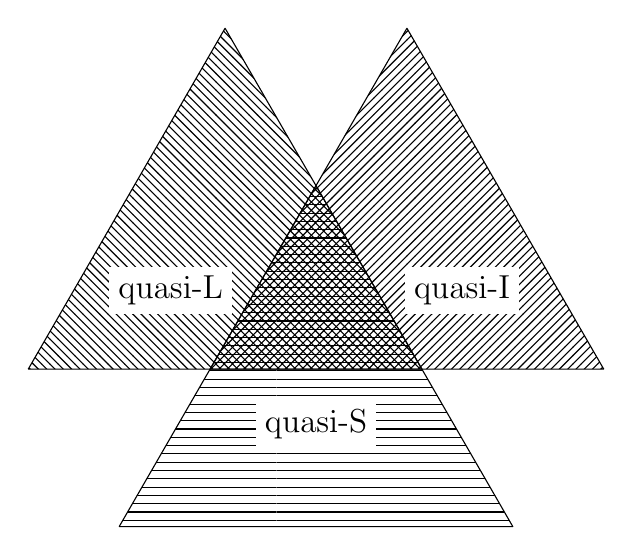
\begin{tikzpicture}[>=latex',line join=bevel,]


\draw[pattern=north east lines] (0,0)--(5,0)--(2.5,4.33)--(0,0);

\draw[pattern=horizontal lines,shift={(-1.1547,-2)}] (0,0)--(5,0)--(2.5,4.33)--(0,0);

\draw[pattern=north west lines,shift={(-2.309401,0)}] (0,0)--(5,0)--(2.5,4.33)--(0,0);

\node[fill=white,shift={(-1.1547,-1.7)}] at (2.5,1) { \large quasi-S };

\node[fill=white] at (3.2,1) { \large quasi-I };
\node[fill=white] at (-0.5,1) { \large quasi-L };

\end{tikzpicture}
}
\end{center}

Basing on this result, the \emph{OM3} class
(symmetric maxitive, minitive, and also modular
aggregation operators) was proposed
in~\cite{CenaGagolewski2013:agop1,CenaGagolewski2013:agop2}.

\bigskip
\begin{definition}
A sequence of nondecreasing functions $\vect{w}=(\func{w}_1,\func{w}_2,\dots)$,
$\func{w}_i :\Ival\to\Ival$,
 and a triangle of coefficients
 $\triangle=(c_{i,n})_{i\in[n],n\in\Naturals}$, $c_{i,n}\in\Ival$
 such that $(\forall n)$ $c_{1,n}\le c_{2,n}\le \dots \le c_{n,n}$,
 $0\le\func{w}_n(0)\le c_{1,n}$, and
 $\func{w}_n(b)=c_{n,n}$,
 generates a nondecreasing \emph{OM3 operator}
 $\func{M}_{\triangle,\vect{w}}:\IvalPow{n}\to\Ival$
 such that for $\vect{x}\in\IvalPow{n}$ we have:
\begin{eqnarray*}
\func{M}_{\triangle,\vect{w}}(\mathbf{x})&=&\bigvee_{i=1}^n
\func{w}_n(x_{(n-i+1)})\wedge c_{i,n} =  \bigwedge_{i=1}^n (\func{w}_n(x_{(n-i+1)}) \vee c_{i-1,n}) \wedge c_{n,n}\\
&=& \sum_{i=1}^n \left(\left(\func{w}_n(x_{(n-i+1)})\vee c_{i-1,n}\right) \wedge
c_{i,n} - c_{i-1,n}\right).
\end{eqnarray*}
\end{definition}
\bigskip

We see that the OM3 class contains i.a.~all
order statistics (whenever $\func{w}_n(x)=x$,
and $c_{i,n}=0$, $c_{j,n}=b$ for $i< k$, $j\ge k$, and some $k$),
OWMax operators (for $\func{w}_n(x)=x$),
and the famous
Hirsch $h$-index (see below).


\subsection{Interesting Impact Functions}

Let us go back to the Producers Assessment Problem.
Below we assume that $\Ival=[0,\infty]$.
% All the functions are symmetric. The input vectors are of course
% being sorted if necessary during calculations.


\paragraph{The $h$-index.}
Given a sequence $\vect{x}=(x_1,\dots,x_n)\in\IvalAnyPow$,
the \emph{Hirsch index} \cite{Hirsch2005:hindex} of $\vect{x}$ is defined as
$\func{H}(\vect{x})=\max\{i=1,\dots,n: x_{\{i\}} \ge i\}$
if $n \ge 1$ and $x_{\{1\}} \ge 1$, or $\func{H}(\vect{x})=0$ otherwise.
It may be shown that the $h$-index is a zero-insensitive
OM3 aggeration operator,
see \cite{Gagolewski2013:om3}, with:
\[
   \func{H}(\vect{x}) = \bigvee_{i=1,\dots,n}^n i\wedge \lfloor x_{\{i\}}\rfloor.
\]
Interpretation: ``an author has $h$-index of $H$ if $H$ of his/her
$n$ most cited papers have at least $H$ citations each, and the other $n-H$
papers are cited no more that $H$ times each''.
The $h$-index may also be expressed as a Sugeno
integral \cite{Sugeno1974:PhD}
w.r.t.~to a counting measure, cf.~\cite{TorraNarukawa2008:h2fuzzyintegrals}
and \cite{GagolewskiMesiar2014:integrals}.

\smallskip
\noindent
\package{agop} implementation: \index{\Rfunc{index\_h()}}\Rfunc{index\_h()}.

\begin{knitrout}\small
\definecolor{shadecolor}{rgb}{0.969, 0.969, 0.969}\color{fgcolor}\begin{kframe}
\begin{alltt}
\hlkwd{index_h}\hlstd{(}\hlkwd{c}\hlstd{(}\hlnum{6}\hlstd{,}\hlnum{5}\hlstd{,}\hlnum{4}\hlstd{,}\hlnum{2}\hlstd{,}\hlnum{1}\hlstd{,}\hlnum{0}\hlstd{,}\hlnum{0}\hlstd{,}\hlnum{0}\hlstd{,}\hlnum{0}\hlstd{,}\hlnum{0}\hlstd{,}\hlnum{0}\hlstd{))}
\end{alltt}
\begin{verbatim}
## [1] 3
\end{verbatim}
\end{kframe}
\end{knitrout}

Moreover, we have $\func{H}(\vect{x})\le \min\{n, x_{1}\}$.

Note that the $h$-index was defined in original context (aggregation
of citation counts) for integer vectors. More generally,
it is better to use the OM3 operator
with $\func{w}_i(x)=x=\mathrm{Id}(x)$
and $c_{i,n}=i$ (two identity ``objects'' = one of the simplest
setting).
Interestingly, such aggregation operator is then
asymptotically idempotent, i.e.~for all $x\in\Ival$
we have $\lim_{n\to\infty} \func{M}_{\triangle,\vect{w}}(n\ast x)=x$.

\paragraph{The $g$-index.}
Egghe's $g$-index \cite{Egghe2006:g}
is defined as
$\func{G}(\vect{x})=\max\{g=1,\dots,n: \sum_{i=1}^g x_{\{g\}}\ge g^2\}$,
and is available in \package{agop} by calling
\index{\Rfunc{index\_g()}}\Rfunc{index\_g()}.
We have $\func{G}(\vect{x})\ge \func{H}(\vect{x})$
with $\func{G}(n\ast n)=\func{H}(n\ast n)=n$


Note that this aggregation operator is not zero-insensitive,
for example $\func{G}(9,0)=2$ and $\func{G}(9,0,0)=3$.
Thus, we also provide the
\index{\Rfunc{index\_g\_zi()}}\Rfunc{index\_g\_zi()} function,
which treats $\vect{x}$ as it would be padded with $0$s.


\begin{knitrout}\small
\definecolor{shadecolor}{rgb}{0.969, 0.969, 0.969}\color{fgcolor}\begin{kframe}
\begin{alltt}
\hlkwd{index_g}\hlstd{(}\hlnum{9}\hlstd{)}
\end{alltt}
\begin{verbatim}
## [1] 1
\end{verbatim}
\begin{alltt}
\hlkwd{index_g}\hlstd{(}\hlkwd{c}\hlstd{(}\hlnum{9}\hlstd{,}\hlnum{0}\hlstd{,}\hlnum{0}\hlstd{))}
\end{alltt}
\begin{verbatim}
## [1] 3
\end{verbatim}
\begin{alltt}
\hlkwd{index_g_zi}\hlstd{(}\hlnum{9}\hlstd{)}
\end{alltt}
\begin{verbatim}
## [1] 3
\end{verbatim}
\end{kframe}
\end{knitrout}

The index is interesting from the computational point of view --
it may be calculated on the nondecreasing vector of cumulative sums,
\texttt{\Rfunc{cumsum}(\Rfunc{sort}(x, \argument{decreasing=}TRUE))},
however, it cannot directly
be expressed as a symmetric maxitive aggregation operator.

However, it might be shown (see \cite{GagolewskiMesiar2014:integrals}
for the proof) that  if $\vect{x}$ is sorted
nondecreasingly, then:
\[
\func{G}(\vect{x}) = \func{H}(\vect{x})(0\vee \mathtt{cummin}(\mathtt{cumsum}(x)-(1:n)^2+(1:n))),
\]
where $1:n = (1, 2, 3, \dots, n)$.

\paragraph{The $w$-index.}
The $w$-index \cite{Woeginger2008:axiomatich}
is  defined as
\begin{equation*}\label{Eq:IndexW}
\func{W}(\vect{x}) = \max\left\{w=0,1,2,\ldots: {x}_{\{i\}} \ge w-i+1, i=1,\dots,w\right\}
\end{equation*}
and is available in \package{agop} by calling
\index{\Rfunc{index\_w()}}\Rfunc{index\_w()}.

Interestingly, we have shown in \cite{GagolewskiMesiar2014:integrals}
that if $\vect{x}$ is sorted nondecreasingly, then:
\[
\func{W}(\vect{x}) = \func{H}(\vect{x})(\mathtt{cummin}(\vect{x}+(1:n)-1)).
\]
Thus, it is easily seen that this is a zero-insensitive impact function.
What is more we have $\func{H}(\vect{x})\le\func{W}(\vect{x})\le 2\func{H}(\vect{x})$
and $\func{W}(\vect{x})\le \min\{n, x_{1}\}$.


\paragraph{The $r_p$-indices.} The $r_p$-index, for $p\geqslant 1$ is expressed as
\[
\func{r}_{p}(\vect{x})=\sup{\{r>0: \func{s}^{p,r}\trianglelefteq\vect{x}\}},
\]
where $\vect{s}^{p,r}=\left(\sqrt[p]{r^p-0^p},\sqrt[p]{r^p-1^p},\dots,
\sqrt[p]{r^p-\lfloor r\rfloor ^p)}\right)$. For more details
see~\cite{Gagolewski2011:PhD,GagolewskiGrzegorzewski2009:geometricapproach}.

Please note that for integer vectors we have $r_1=\func{W}$ and $r_\infty=\func{H}$
(cf.~\cite{GagolewskiGrzegorzewski2009:geometricapproach}).
Hence it easily seen that, this is a zero-insensitive impact function.

\package{agop} implementation: \index{\Rfunc{index\_rp()}}\Rfunc{index\_rp()}.

\paragraph{The $l_p$-indices.} The $l_p$-index
(cf.~\cite{Gagolewski2011:PhD,GagolewskiGrzegorzewski2009:geometricapproach})
for $p\in[1,\infty)$, $u>0$ and $v>0$ is a function
$\func{l}_{p}:\IvalAnyPow\to\IvalPow{2}$ given by the equation
\[
\func{l}_{p}(\vect{x})=\mathrm{arg}\sup_{(u,v)}{\{uv: \func{e}^{p,u,v}\trianglelefteq\vect{x}\}},
\]
where $\func{e}^{p,u,v}=\left(\sqrt[p]{v^{p}-(\frac{v}{u}0)^{p}},
\sqrt[p]{v^{p}-(\frac{v}{u}1)^{p}},\dots,\sqrt[p]{v^{p}-(\frac{v}{u}\lfloor u\rfloor)^{p}}\right)$.

\package{agop} implementation: \index{\Rfunc{index\_lp()}}\Rfunc{index\_lp()}.



\paragraph{The $\mathrm{MAXPROD}$-index.}
The MAXPROD-index \cite{Kosmulski2007:maxprod} is given  by the equation
\begin{equation*}\label{Eq:IndexMaxProd}
   \func{MP}(\vect{x}) = \max\left\{i\cdot{{x}}_{\{i\}}: i=1,2,\ldots\right\}
\end{equation*}
is another example of zero-insensitive impact function.
Interestingly, this index is a particular case of a projected $l_\infty$-index,
see~\cite{GagolewskiGrzegorzewski2009:geometricapproach}, and can be also expressed
in terms of Shilkret integral \cite{Shilkret1971:maxitivemeasure},
see \cite{GagolewskiMesiar2014:integrals} for discussion.

In \package{agop} the MAXPROD-index is implemented
in the \index{\Rfunc{index\_maxprod()}}\Rfunc{index\_maxprod()} function.



\paragraph{Simple transformations of the $h$-index.}
Bibliometricians in many papers considered very
simple, direct modifications of the $h$-index.
For example, the $h(2)$-index \cite{Kosmulski2006:h2}
is defined as:
\begin{equation*}\label{Eq:IndexH2}
\func{H2}(\vect{x}) = \max\left\{h=0,1,2,\ldots: {x}_{h} \ge h^2\right\}. %= \left\lfloor \bigvee_{i=1,2,\dots} i\wedge x_{i}\right\rfloor
\end{equation*}
Some authors introduced other settings than ``$h^2$'' on the right
side of \eqref{Eq:IndexH2}, e.g. ``$2h$'', ``$\alpha h$'' for some
$\alpha > 0$, or ``$h^\beta$'', $\beta\ge 1$, cf.~\cite{AlonsoETAL2009:hreview}.

It may easily be shown that these reduce to the $h$-index for
properly transformed input vectors,
e.g.~$\func{H2}(\vect{x})=\func{H}(\sqrt{\vect{x}})$.



\subsection{Noteworthy Fuzzy Logic Connectives}

All the predefined fuzzy logic connectives have been vectorized in \package{agop}.
In other words, any e.g.~binary operation $B: [0,1]^2\to [0,1]$ has
been extended to act on vectors of arbitrary length.
Given $\vect{x},\vect{y}\in[0,1]^n$ we have
$B(\vect{x},\vect{y})=(B(x_1, y_1), \dots, B(x_n, y_n))$.
For instance:

\begin{knitrout}\small
\definecolor{shadecolor}{rgb}{0.969, 0.969, 0.969}\color{fgcolor}\begin{kframe}
\begin{alltt}
\hlstd{x} \hlkwb{<-} \hlkwd{c}\hlstd{(}\hlnum{0}\hlstd{,} \hlnum{0.5}\hlstd{,} \hlnum{1}\hlstd{)}
\hlstd{y} \hlkwb{<-} \hlkwd{c}\hlstd{(}\hlnum{0.4}\hlstd{,} \hlnum{0.6}\hlstd{,} \hlnum{0.8}\hlstd{)}
\hlkwd{tnorm_lukasiewicz}\hlstd{(x, y)}
\end{alltt}
\begin{verbatim}
## [1] 0.0 0.1 0.8
\end{verbatim}
\end{kframe}
\end{knitrout}

Note that many new logical connectives may be generated via existing ones.
For example, given any fuzzy implication $I$, $N(x)=I(x,0)$ is a fuzzy negation.
Moreover, given any t-conorm $S$ and any negation $N$, $I(x, y)=S(N(x), y)$
is a fuzzy implication (a so-called (S-N)-implication),
see e.g.~\cite{BaczynskiJayaram2008:fuzzyimplications} for more details.

And here is how we may create exemplary contour plots of various t-norms:

\begin{knitrout}\small
\definecolor{shadecolor}{rgb}{0.969, 0.969, 0.969}\color{fgcolor}\begin{kframe}
\begin{alltt}
\hlstd{x} \hlkwb{<-} \hlkwd{seq}\hlstd{(}\hlnum{0}\hlstd{,} \hlnum{1}\hlstd{,} \hlkwc{length.out}\hlstd{=}\hlnum{100}\hlstd{)}
\hlstd{y} \hlkwb{<-} \hlkwd{seq}\hlstd{(}\hlnum{0}\hlstd{,} \hlnum{1}\hlstd{,} \hlkwc{length.out}\hlstd{=}\hlnum{100}\hlstd{)}
\hlkwd{par}\hlstd{(}\hlkwc{mfrow}\hlstd{=}\hlkwd{c}\hlstd{(}\hlnum{2}\hlstd{,}\hlnum{2}\hlstd{))}
\hlstd{funs} \hlkwb{<-} \hlkwd{list}\hlstd{(}\hlstr{"Minimum t-norm"}\hlstd{=tnorm_minimum,} \hlstr{"Product t-norm"}\hlstd{=tnorm_product,}
             \hlstr{"Lukasiewicz t-norm"}\hlstd{=tnorm_lukasiewicz,} \hlstr{"Drastic t-norm"}\hlstd{=tnorm_drastic)}
\hlkwa{for} \hlstd{(i} \hlkwa{in} \hlkwd{seq_along}\hlstd{(funs)) \{}
   \hlstd{z} \hlkwb{<-} \hlkwd{outer}\hlstd{(x, y, funs[[i]])}
   \hlkwd{image}\hlstd{(x, y, z,} \hlkwc{col}\hlstd{=}\hlkwd{heat.colors}\hlstd{(}\hlnum{20}\hlstd{))}
   \hlkwd{title}\hlstd{(}\hlkwc{main}\hlstd{=}\hlkwd{names}\hlstd{(funs)[i])}
   \hlkwd{contour}\hlstd{(x, y, z,} \hlkwc{nlevels}\hlstd{=}\hlnum{25}\hlstd{,} \hlkwc{add}\hlstd{=}\hlnum{TRUE}\hlstd{)}
\hlstd{\}}
\end{alltt}
\end{kframe}
\end{knitrout}

\begin{center}
% \scalebox{0.83}{
\begin{knitrout}\small
\definecolor{shadecolor}{rgb}{0.969, 0.969, 0.969}\color{fgcolor}

{\centering \includegraphics[width=4.5in]{figures-knitr/tnorms_plot2} 

}



\end{knitrout}
% }
\end{center}

\noindent
For 3D plots, check out e.g.~the \package{plot3D} package.


\paragraph{t-norms}

Table \ref{Tab:tnorms} lists all the t-norms predefined by the \package{agop} package.
For any t-norm $T$ and all $x,y$ it holds $T_\mathrm{D}(x,y)\le T(x,y)\le T_\mathrm{M}(x, y)$.
Moreover, we have $T_\mathrm{Ł}(x,y)\le T_\mathrm{P}(x,y)$.

\begin{table}[htb!]
\caption{\label{Tab:tnorms} Exemplary t-norms}
\centering
\begin{tabular}{llp{7cm}}
\hline
\bf Name & \bf Function & \bf Definition \\
\hline
\hline
Minimum & \index{\Rfunc{tnorm\_minimum()}}\Rfunc{tnorm\_minimum()} & $T_\mathrm{M}(x, y)=x\wedge y$ \\
Product & \index{\Rfunc{tnorm\_product()}}\Rfunc{tnorm\_product()} & $T_\mathrm{P}(x, y)=xy$ \\
Łukasiewicz & \index{\Rfunc{tnorm\_lukasiewicz()}}\Rfunc{tnorm\_lukasiewicz()} & $T_\mathrm{Ł}(x, y)=(x+y-1)\vee 0$ \\
Drastic & \index{\Rfunc{tnorm\_drastic()}}\Rfunc{tnorm\_drastic()} & $$T_\mathrm{D}(x, y)=\left\{
\begin{array}{ll}
0 & \text{if }x, y\in[0,1)\\
x\wedge y & \text{if }x=1\text{ or }y=1\\
\end{array}
\right.$$ \\
Fodor & \index{\Rfunc{tnorm\_fodor()}}\Rfunc{tnorm\_fodor()} & $$T_\mathrm{F}(x, y)=\left\{
\begin{array}{ll}
0 & \text{if }x+y\le 1\\
x\wedge y & \text{if }x+y>1\\
\end{array}
\right.$$ \\
\hline
\end{tabular}
\end{table}


\paragraph{t-conorms}

Table \ref{Tab:tconorms} lists all the t-conorms in the \package{agop} package.
For any t-conorm $S$ and all $x,y$ it holds $S_\mathrm{M}(x,y)\le T(x,y)\le S_\mathrm{D}(x, y)$.
Moreover, we have $S_\mathrm{P}(x,y)\le S_\mathrm{Ł}(x,y)$.
Also note that $S$ is a t-conorm if and only if there exists a t-norm $t$
such that for all $x,y$ it holds
$S(x,y)=1-T(1-x, 1-y)$, see \cite{KlementMesiarPap2000:trinorm}.

\begin{table}[htb!]
\caption{\label{Tab:tconorms} Exemplary t-conorms}
\centering
\begin{tabular}{llp{7cm}}
\hline
\bf Name & \bf Function & \bf Definition \\
\hline
\hline
Maximum & \index{\Rfunc{tconorm\_minimum()}}\Rfunc{tconorm\_minimum()} & $S_\mathrm{M}(x, y)=x\vee y$ \\
Product & \index{\Rfunc{tconorm\_product()}}\Rfunc{tconorm\_product()} & $S_\mathrm{P}(x, y)=x+y-xy$ \\
Łukasiewicz & \index{\Rfunc{tconorm\_lukasiewicz()}}\Rfunc{tconorm\_lukasiewicz()} & $S_\mathrm{Ł}(x, y)=(x+y)\wedge 1$ \\
Drastic & \index{\Rfunc{tconorm\_drastic()}}\Rfunc{tconorm\_drastic()} & $$S_\mathrm{D}(x, y)=\left\{
\begin{array}{ll}
1 & \text{if }x, y\in(0,1]\\
x\vee y & \text{if }x=0\text{ or }y=0\\
\end{array}
\right.$$ \\
Fodor & \index{\Rfunc{tconorm\_fodor()}}\Rfunc{tconorm\_fodor()} & $$S_\mathrm{F}(x, y)=\left\{
\begin{array}{ll}
1 & \text{if }x+y\ge 1\\
x\vee y & \text{if }x+y<1\\
\end{array}
\right.$$ \\
\hline
\end{tabular}
\end{table}





\paragraph{Fuzzy negations}

Table~\ref{Tab:fnegations} lists available fuzzy negations.
For any $N$ and $x$ it holds $N_0(x)\le N(x)\le N_1(x)$.


\begin{table}[htb!]
\caption{\label{Tab:fnegations} Exemplary fuzzy negations}
\centering
\begin{tabular}{llp{7cm}}
\hline
\bf Name & \bf Function & \bf Definition \\
\hline
\hline
Classic & \index{\Rfunc{fnegation\_classic()}}\Rfunc{fnegation\_classic()} & $N_\mathrm{C}(x)=1-x$ \\
minimal & \index{\Rfunc{fnegation\_minimal()}}\Rfunc{fnegation\_minimal()} & $$N_0(x)=\left\{
\begin{array}{ll}
1 & \text{if }x=0\\
0 & \text{if }x>0\\
\end{array}
\right.$$ \\
maximal & \index{\Rfunc{fnegation\_maximal()}}\Rfunc{fnegation\_maximal()} & $$N_1(x)=\left\{
\begin{array}{ll}
1 & \text{if }x<1\\
0 & \text{if }x=1\\
\end{array}
\right.$$ \\
Yager & \index{\Rfunc{fnegation\_yager()}}\Rfunc{fnegation\_yager()} & $N_\mathrm{Y}(x)=\sqrt{1-x^2}$ \\
\hline
\end{tabular}
\end{table}





\paragraph{Fuzzy implications}


Table~\ref{Tab:fimplications} lists fuzzy implications predefined in \package{agop}.
For any $I$ and $x,y$ it holds $I_0(x,y)\le I(x,y)\le I_1(x,y)$.

\begin{table}[htb!]
\caption{\label{Tab:fimplications} Exemplary fuzzy implications}
\centering
\begin{tabular}{llp{7cm}}
\hline
\bf Name & \bf Function & \bf Definition \\
\hline
\hline
minimal & \index{\Rfunc{fimplication\_minimal()}}\Rfunc{fimplication\_minimal()} & $$I_0(x,y)=\left\{
\begin{array}{ll}
1 & \text{if }x=0\text{ or }y=1\\
0 & \text{otherwise}\\
\end{array}
\right.$$ \\
maximal & \index{\Rfunc{fimplication\_maximal()}}\Rfunc{fimplication\_maximal()} & $$I_1(x,y)=\left\{
\begin{array}{ll}
0 & \text{if }x=1\text{ and }y=0\\
1 & \text{otherwise}\\
\end{array}
\right.$$ \\
Kleene-Dienes & \index{\Rfunc{fimplication\_kleene()}}\Rfunc{fimplication\_kleene()} & $I_\mathrm{KD}(x,y)=(1-x)\vee y$ \\
Łukasiewicz & \index{\Rfunc{fimplication\_lukasiewicz()}}\Rfunc{fimplication\_lukasiewicz()} & $I_\mathrm{Ł}(x,y)=(1-x+y)\wedge 1$ \\
Reichenbach & \index{\Rfunc{fimplication\_reichenbach()}}\Rfunc{fimplication\_reichenbach()} & $I_\mathrm{RB}(x,y)=1-x+xy$ \\
Fodor & \index{\Rfunc{fimplication\_fodor()}}\Rfunc{fimplication\_fodor()} & $$I_\mathrm{F}(x,y)=\left\{
\begin{array}{ll}
1 & \text{if }x\le y\\
(1-x)\vee y & \text{if }x> y\\
\end{array}
\right.$$ \\
Goguen & \index{\Rfunc{fimplication\_goguen()}}\Rfunc{fimplication\_goguen()} & $$I_\mathrm{GG}(x,y)=\left\{
\begin{array}{ll}
1  & \text{if }x\le y\\
y/x  & \text{if }x> y\\
\end{array}
\right.$$ \\
G\"{o}del & \index{\Rfunc{fimplication\_goedel()}}\Rfunc{fimplication\_goedel()} & $$I_\mathrm{GD}(x,y)=\left\{
\begin{array}{ll}
1  & \text{if }x\le y\\
y  & \text{if }x> y\\
\end{array}
\right.$$ \\
Rescher & \index{\Rfunc{fimplication\_rescher()}}\Rfunc{fimplication\_rescher()} & $$I_\mathrm{RS}(x,y)=\left\{
\begin{array}{ll}
1  & \text{if }x\le y\\
0  & \text{if }x> y\\
\end{array}
\right.$$ \\
Weber & \index{\Rfunc{fimplication\_weber()}}\Rfunc{fimplication\_weber()} & $$I_\mathrm{W}(x,y)=\left\{
\begin{array}{ll}
1 & \text{if }x<1\\
y & \text{if }x=1\\
\end{array}
\right.$$ \\
Yager & \index{\Rfunc{fimplication\_yager()}}\Rfunc{fimplication\_yager()} & $$I_\mathrm{Y}(x,y)=\left\{
\begin{array}{ll}
1 & \text{if }x=0\text{ and }y=0\\
y^x & \text{otherwise}\\
\end{array}
\right.$$ \\
\hline
\end{tabular}
\end{table}

\subsection{A Note on Copulas}

Copulas are used in probability and statistics
to model dependency between random variables (cf.~the Sklar theorem).
Many copulas are defined e.g.~by the \package{copula} package
-- we decided not to duplicate its features.

\begin{knitrout}\small
\definecolor{shadecolor}{rgb}{0.969, 0.969, 0.969}\color{fgcolor}\begin{kframe}
\begin{alltt}
\hlkwd{library}\hlstd{(}\hlstr{"copula"}\hlstd{)}
\hlstd{cc} \hlkwb{<-} \hlkwd{frankCopula}\hlstd{(}\hlnum{1}\hlstd{,} \hlkwc{dim}\hlstd{=}\hlnum{2}\hlstd{)}
\hlkwd{pCopula}\hlstd{(}\hlkwd{c}\hlstd{(}\hlnum{0.5}\hlstd{,} \hlnum{0.8}\hlstd{), cc)} \hlcom{# 0.4197217}
\hlkwd{pCopula}\hlstd{(}\hlkwd{c}\hlstd{(}\hlnum{0.9}\hlstd{,} \hlnum{1.0}\hlstd{), cc)} \hlcom{# 0.9}
\end{alltt}
\end{kframe}
\end{knitrout}

Note that t-norms such as $T_\mathrm{M}, T_\mathrm{P},$ and $T_\mathrm{Ł}$
are examples of 2-copulas.
On the other hand, $T_\mathrm{D}$ and $T_\mathrm{F}$ are not 2-copulas.

Interestingly, by the Frechet-Hoefding theorem,
we have $T_\mathrm{Ł}(x, y)\le C(x,y)\le T_\mathrm{M}(x,y)$ for
any $x,y$ and 2-copula $C$, see e.g.~\cite{KlementMesiarPap2000:trinorm}.

\subsection{Interesting Spread Measures}

.....
(see \Rfunc{var()}), standard deviation
(see \Rfunc{sd()}), range, interquartile range
(IQR, see \Rfunc{IQR()}),
median absolute deviation (MAD, see \Rfunc{mad()}) etc., that is
functions widely used in exploratory data analysis
as descriptive statistics.

...TO DO...

D2OWA (\index{\Rfunc{d2owa()}}\Rfunc{d2owa()}):

\[
\func{D2OWA}_\vect{w}(\vect{x}) = \sqrt{\frac{1}{n}
   \sum_{i=1}^n \left(x_i-\func{OWA}_\vect{w}(\vect{x})\right)^2}
\]


%%%%%%%%%%%%%%%%%%%%%%%%%%%%%%%%%%%%%%%%%%%%%%%%%%%%%%%%%%%%%%%%%%%%%
%%%%%%%%%%%%%%%%%%%%%%%%%%%%%%%%%%%%%%%%%%%%%%%%%%%%%%%%%%%%%%%%%%%%%
%%%%%%%%%%%%%%%%%%%%%%%%%%%%%%%%%%%%%%%%%%%%%%%%%%%%%%%%%%%%%%%%%%%%%



\section{Aggregation Operators from the Probabilistic Perspective}

By default, theory of aggregation looks at the aggregation operators
mainly from the algebraic perspective. Of course, we may also
be interested in their probabilistic properties,
e.g.~in i.i.d.~RVs models (the simplest and the most ``natural''
ones in statistics), cf.~\cite{Gagolewski2011:PhD} for discussion.

Intuitively, a random variable is a method for ``producing''
input data. An aggregation operator applied on a random variable
(possibly multidimensional) is classically called a~\emph{statistic}.




\subsection{Some Notable Probability Distributions}

Let $(X_1,\dots,X_n)$ i.i.d.~$F$, where $\mathrm{supp}\,F = \Ival$.
In social phenomena modeling, if $F$ is continuous,
we often assume that the underlying density $f$ is decreasing
and convex on $\Ival$, possibly with heavy-tails.
E.g.~in the bibliometric impact assessment problem,
this assumption reflects the fact that higher paper valuations
are more difficult to obtain than the lower ones,
most of the papers have very small valuation (near $0$),
and the probability of attaining a high note decreases in at least
linear pace.

Let us make a review of some useful statistical
distributions, that are not available through ``base'' \R
(for other ones, e.g.~exponential, normal, uniform, Weibull, etc.~refer
to the widely-available literature).



\subsubsection{Pareto-Type II Distribution}

Many generalizations of the Pareto distribution
have been proposed (GPD, \textit{Generalized Pareto Distributions},
cf.~e.g.~\cite{VillasenorGonzalez2009:gofgpd,Zhang2010:estgpd}).
Here we will introduce the so-called Pareto-Type II (Lomax) distribution,
which has support $\Ival=[0,\infty]$
and is defined with two parameters.


Formally, $X$ follows the Pareto-II distribution
with shape parameter $k>0$ and scale parameter $s>0$,
denoted $X\sim\mathrm{P2}(k,s)$, if its density is of the form
\begin{equation}\label{Eq:Pareto2PDF}
   f(x)=\frac{k s^k}{(s+x)^{k+1}}\quad (x\ge 0).
\end{equation}
The cumulative distribution function of $X$ is then:
\begin{equation}\label{Eq:Pareto2CDF}
   F(x) = 1-\dfrac{s^k}{(s+x)^k}\quad (x\ge 0).
\end{equation}

The Pareto-Type II distribution
is implemented in \package{agop}:
\index{\Rfunc{dpareto2()}}\Rfunc{dpareto2()} gives the p.d.f.~\eqref{Eq:Pareto2PDF},
\index{\Rfunc{ppareto2()}}\Rfunc{ppareto2()} gives the c.d.f.~\eqref{Eq:Pareto2CDF},
\index{\Rfunc{qpareto2()}}\Rfunc{qpareto2()} calculates the quantile function, $F^{-1}$,
and \index{\Rfunc{rpareto2()}}\Rfunc{rpare\-to2()} generates random deviates.

\paragraph{Properties.}
The expected value of $X\sim\mathrm{P2}(k,s)$
exists for $k>1$ and is equal to
\(\mathbb{E}X = \frac{s}{k-1}.\)
Variance exists for $k>2$ and is equal to
\(\mathrm{Var}\, X = \frac{ks^2}{(k-2)(k-1)^2}.\)
More generally, the $i$-th raw moment for $k>i$ is given by:
\(\mathbb{E}X^i = \frac{\Gamma(i+1)\Gamma(k-i)}{\Gamma(k+1)} ks^i.\)

For a fixed $s$, if $X\sim \mathrm{P2}(k_x,s)$ and $Y\sim \mathrm{P2}(k_y,s)$,
$k_x<k_y$, then $X$ stochastically dominates $Y$,
denoted $X\succ Y$.
On the other hand, for a fixed $k$, if $X\sim \mathrm{P2}(k,s_x)$
and $Y\sim \mathrm{P2}(k,s_y)$, then $s_x>s_y$ implies $X \succ Y$.

Most importantly, if $X\sim\mathrm{P2}(k,s)$,
then the conditional distribution of $X-t$ given $X>t$,
is $\mathrm{P2}(k,s+t)$ $t \ge 0$.

Additionally, it might be shown that if $X\sim\mathrm{P2}(k,s)$,
then $\ln(s+X)$ has c.d.f.~$F(x)=1-s^k e^{-kx}$ and
density $f(x)=k s^k e^{-kx}$ for $x\ge\ln s$,
i.e. has the same distribution as $Z+\ln s$, where
$Z\sim\mathrm{Exp}(k)\equiv \Gamma(1,1/k)$
(exponential distribution).




\paragraph{Parameter estimation.}
Let $\vect{x}=(x_1,\dots,x_n)$ be a realization of the Pareto-Type II
i.i.d. sample with known $s>0$.
The unbiased (corrected) maximum likelihood estimator for $k$:
% rozk³adu Pareto II rodzaju mo¿na próbowaæ wyznaczyæ metod±
% najwiêkszej wiarogodno¶ci (MLE).
% Logarytm funkcji wiarogodno¶ci dany jest wzorem
% \begin{eqnarray}
% \ln \mathcal{L}(k,s;\vect{x}) &=& n\ln k + nk\ln s - (k+1)\sum_{i=1}^n \ln(s+x_i) \\
%                               &=& n\ln k - n\ln\tfrac{1}{s}  - (k+1)\sum_{i=1}^n \ln(1+\tfrac{1}{s} x_i).
% \end{eqnarray}
%
% Dla znanego $s>0$ i~danej realizacji próby $(x_1,\dots,x_n)$ mamy
% \begin{equation}
% \widehat{k}=\dfrac{n}{\sum_{i=1}^n \ln\left(1+\tfrac{1}{s} x_i\right)}.
% \end{equation}
% For $n>2$ zachodzi
% \begin{eqnarray*}
% \mathbb{E}\widehat{k} &=& k \dfrac{n}{n-1},\\
% \mathrm{Var}\,\widehat{k}&=&k^2 \frac{n^2}{(n-2) (n-1)^2},
% \end{eqnarray*}
% jest to zatem  tylko asymptotycznie nieobci±¿ony estymator parametru $k$.
% £atwo jednak uwzglêdniæ poprawkê na nieobci±¿ono¶æ: \marginpar{Nieobci±¿ony estymator MLE: $\widehat{k}_{\mathrm{MLEU}}$}
\begin{equation*}
\widehat{k}(\vect{x})=\dfrac{n-1}{\sum_{i=1}^n \ln\left(1+\tfrac{1}{s} x_i\right)}.
\end{equation*}
It may be shown that for $n>2$ it holds
$\mathrm{Var}\,\widehat{k}(\vect{x})=k^2 \frac{1}{n-2}.$


\package{agop} implementation:
\index{\Rfunc{pareto2\_estimate\_mle()}}\Rfunc{pareto2\_estimate\_mle()}
with explicitly set argument \argument{s}.

\begin{knitrout}\small
\definecolor{shadecolor}{rgb}{0.969, 0.969, 0.969}\color{fgcolor}\begin{kframe}
\begin{alltt}
\hlkwd{rowMeans}\hlstd{(}\hlkwd{replicate}\hlstd{(}\hlnum{1000}\hlstd{, \{}
   \hlkwd{pareto2_estimate_mle}\hlstd{(}\hlkwd{rpareto2}\hlstd{(}\hlnum{50}\hlstd{,} \hlnum{2}\hlstd{,} \hlnum{1.5}\hlstd{),} \hlkwc{s}\hlstd{=}\hlnum{1.5}\hlstd{)}
\hlstd{\}))}
\end{alltt}
\begin{verbatim}
##        k        s 
## 1.988461 1.500000
\end{verbatim}
\end{kframe}
\end{knitrout}

\bigskip
For both unknown $k$ and $s$ we have:
\begin{equation*}\label{Eq:rownaniapochMLE}
\left\{
\begin{array}{lll}
\widehat{k} = \frac{n}{\sum_{i=1}^n \ln\left(1+x_i/\widehat{s}\right)}, \\
1+\frac{1}{n} \sum_{i=1}^n \ln\left(1+x_i/\widehat{s}\right) - \frac{n}{\sum_{i=1}^n \left(1+x_i/\widehat{s}\right)^{-1}}  &=& 0. \\
\end{array}\right.
\end{equation*}
Unfortunately, the second equation must be solved numerically.
It is worth noting that the above system of equations may sometimes
have no solution (as the local minimum of the likelihood function may not exist,
see \cite{CastilloDaoudi2009:mlegpd} for discussion).
This estimator may be heavily biased and have a large mean squared
error (of course, it is only asymptotically unbiased).

\package{agop} implementation:
\index{\Rfunc{pareto2\_estimate\_mle()}}\Rfunc{pareto2\_estimate\_mle()} with explicitly
set argument \argument{s}.

\begin{knitrout}\small
\definecolor{shadecolor}{rgb}{0.969, 0.969, 0.969}\color{fgcolor}\begin{kframe}
\begin{alltt}
\hlkwd{rowMeans}\hlstd{(}\hlkwd{replicate}\hlstd{(}\hlnum{1000}\hlstd{, \{}
   \hlkwd{pareto2_estimate_mle}\hlstd{(}\hlkwd{rpareto2}\hlstd{(}\hlnum{50}\hlstd{,} \hlnum{2}\hlstd{,} \hlnum{1.5}\hlstd{))}
\hlstd{\}),} \hlkwc{na.rm}\hlstd{=}\hlnum{TRUE}\hlstd{)}
\end{alltt}
\begin{verbatim}
##        k        s 
## 2.876271 2.418572
\end{verbatim}
\end{kframe}
\end{knitrout}

\noindent
We see that the estimator's performance is weak.

A better (in general) estimation procedure was proposed
in \cite{ZhangStevens2009:estgpd}.
The Zhang-Stevens MMS (\textit{minimum mean square error}) (Bayesian)
estimator has relatively small bias (often positive) and mean squared error.
In \package{agop} it is available as:
\index{\Rfunc{pareto2\_estimate\_mmse()}}\Rfunc{pareto2\_estimate\_mmse}.

\begin{knitrout}\small
\definecolor{shadecolor}{rgb}{0.969, 0.969, 0.969}\color{fgcolor}\begin{kframe}
\begin{alltt}
\hlkwd{suppressWarnings}\hlstd{(}\hlkwd{rowMeans}\hlstd{(}\hlkwd{replicate}\hlstd{(}\hlnum{1000}\hlstd{, \{}
   \hlkwd{pareto2_estimate_mmse}\hlstd{(}\hlkwd{rpareto2}\hlstd{(}\hlnum{50}\hlstd{,} \hlnum{2}\hlstd{,} \hlnum{1.5}\hlstd{))}
\hlstd{\})))}
\end{alltt}
\begin{verbatim}
##        k        s 
## 4.037108 3.291486
\end{verbatim}
\end{kframe}
\end{knitrout}

% W~przypadku niemo¿liwo¶ci obliczenia warto¶ci estymatorów metod± najwiêkszej
% wiarogodno¶ci powinni¶my u¿yæ innego estymatora.
% Metoda momentów nie jest polecana, gdy¿ momenty zwyk³e rzêdu $i$, jak wspomniano
% wy¿ej, s± okre¶lone tylko dla $k>i$.
% Co wiêcej,  w~przypadku niektórych zaobserwowanych warto¶ci $\vect{x}$,
% równie¿ estymatory wyznaczone metod± kwantyli mog± nie byæ wyznaczalne.
% Inne, bardziej skomplikowane metody zosta³y opisane m.in.~w~pracach
% \cite{ZeaKots2001:estgpd,Luceno2006:estgpd,Zhang2010:estgpd}.
% Jak pokazuj± wyniki symulacyjne, dla nieznanego zarówno parametru
% $k$ jak i~$s$, estymatory te cechuj± siê lepszymi w³asno¶ciami ni¿ estymator
% najwiêkszej wiarogodno¶ci.
%
% \bigskip\label{Ozn:MMSE}
% Warto zwróciæ szczególn± uwagê na metodê szacowania warto¶ci parametrów zaproponowan±
% przez Zhanga i Stevensa \cite{ZhangStevens2009:estgpd}.
% Przedstawiany estymator
% cechuje siê niewielkim obci±¿eniem (najczê¶ciej
% dodatnim), wzglêdnie ma³± wariancj± oraz tym, ¿e da siê
% wyznaczyæ jego warto¶æ w~prawie wszystkich przypadkach.



% Niech $\theta := -\frac{1}{s}$, gdzie
% $-1\le \theta < 0$.
% Poszukujemy estymatora bayesowskiego minimalizuj±cego ¶redniokwadratow±
% funkcjê ryzyka
% (estymator MMSE, ang. \textit{minimum mean square error estimator}),
% który jest warto¶ci± oczekiwan± rozk³adu a~posteriori
% \begin{equation}\label{Eq:MMSEbayes}
% \widehat{\theta} = \Expectation(\theta | \vect{X}=\vect{x}) = \int_{-1}^0 \theta\, \pi(\theta|\vect{x})\,d\theta,
% \end{equation}
% gdzie
% \begin{equation}
% \pi(\theta|\vect{x})=\frac{h(\theta; \vect{x}) \exp[{\ell(\theta; \vect{x})}]}{\int_{-1}^0 h(\theta; \vect{x}) \exp[{\ell(\theta; \vect{x})}]  \,d\theta},
% \end{equation}
% dla  pewnej gêsto¶ci rozk³adu
% a~priori $h(\theta; \vect{x})$ oraz
% logarytmu z~profilowej funkcji wiarogodno¶ci (ang. \textit{profile log-likelihood})
% parametru $\theta$ postaci
% \[\ell(\theta; \vect{x}):=n\left( \ln(-{k}^*\theta)-1-1/{k}^* \right),\]
% gdzie
% \[{k}^* = n \left[\sum_{i=1}^n \ln\left(1-\theta x_i\right) \right]^{-1}.\]
%
% W~rozpatrywanej pracy stosowane jest nastêpuj±ce
% przybli¿enie numeryczne wzoru \eqref{Eq:MMSEbayes}.
% Dla $m=20+\lfloor n\rfloor$ i~$j=1,\dots,m$ niech
% \[
% \vartheta_j = 1/x_{(n)} + \left[ 1-\sqrt{\frac{m}{j-0{,}5}} \right] \textfractionsolidus (3\, x_{(\lfloor n/4+0.5\rfloor)}).
% \]
% \clearpage\noindent
% Ponadto, niech $w(\vartheta_j) = \exp(\ell(\vartheta_j; \vect{x}))/\sum_{i=1}^{m} \exp(\ell(\vartheta_i;\vect{x}))$.
% W~konsekwencji, estymatorem parametru skali bêdzie
% $
%    \widehat{s}_\text{ZS} = -1/\sum_{j=1}^m \vartheta_j w(\vartheta_j).
% $
% Warto¶æ $\widehat{k}_\text{ZS}$ wyznaczamy z~pierwszego równania                \marginpar{Estymatory MMSE: $\widehat{k}_\text{ZS}$~i~$\widehat{s}_\text{ZS}$}
% uk³adu \eqref{Eq:rownaniapochMLE}.
% Jako rozk³adu a~priori $h(\theta; \vect{x})$ u¿ywamy tutaj
% gêsto¶ci rozk³adu $\mathrm{P2}(2, 1/3\, x_{(\lfloor n/4+0.5\rfloor)})$
% (por.~motywacjê i~dyskusjê w~\cite{ZhangStevens2009:estgpd}).
% Algorytm wyznaczaj±cy estymatory przedstawion± metod±
% zosta³ zaimplementowany w~bibliotece \CITAN{} w~funkcji \Rfunc{pareto2.zsestimate()},
% zob.~rozdz.~\ref{Func:pareto2.zsestimate}.
%

\paragraph{Goodness-of-fit tests.}
\index{\Rfunc{pareto2\_test\_ad()}}\Rfunc{pareto2\_test\_ad()} ..... -- Anderson-Darling goodness-of-fit
test (approximate p-value)..... (TO DO: describe)
for known $s$
by means of the
\index{\Rfunc{exp\_test\_ad()}}\Rfunc{exp\_test\_ad()} function and
the above-mentioned relationship between Pareto-Type II distributions
and Exponential ones.

\begin{knitrout}\small
\definecolor{shadecolor}{rgb}{0.969, 0.969, 0.969}\color{fgcolor}\begin{kframe}
\begin{alltt}
\hlstd{x} \hlkwb{<-} \hlkwd{rpareto2}\hlstd{(}\hlnum{100}\hlstd{,} \hlkwc{k}\hlstd{=}\hlnum{1}\hlstd{,} \hlkwc{s}\hlstd{=}\hlnum{2}\hlstd{)}
\hlkwd{pareto2_test_ad}\hlstd{(x,} \hlkwc{s}\hlstd{=}\hlnum{2}\hlstd{)}
\end{alltt}
\begin{verbatim}
## 
## 	Anderson-Darling goodness-of-fit test for Pareto Type-II
## 	distribution
## 
## data:  x
## W = 0.3169, p-value = 0.797
\end{verbatim}
\end{kframe}
\end{knitrout}


% \paragraph{Testowanie zgodno¶ci.}\label{Ozn:P2GoF}
% Przedstawione estymatory mog± byæ u¿yte                                         \marginpar{GoF}
% w~procedurze  testowania zgodno¶ci %(ang. \textit{goodness-of-fit tests})
% danej zaobserwowanej próbki losowej z~rozk³adem Pareto II rodzaju.
% W~tym celu mo¿na u¿yæ np. testu Ko³mogorowa,
% Cram\'{e}ra-von Misesa b±dŒ Andersona-Darlinga (który przyk³ada wiêksz± wagê
% od pozosta³ych do obserwacji w~ogonach rozk³adu),
% por.~analizê w³asno¶ci tych testów w~pracach \cite{ChoulakianStephens2001:gofgpd,
% ZhangStevens2009:estgpd}.
%
% W~bibliotece \CITAN{} udostêpnili¶my funkcjê funkcjê \Rfunc{pareto2.gof\-test()}
% (zob. rozdz.~\ref{Func:pareto2.goftest}),
% która domy¶lnie stosuje test Andersona-Darlinga,
% w~którym rozk³ad statystyki przybli¿ony jest za pomoc± metody zaproponowanej
% w~\cite{MarsagliaMarsaglia2004:adtest}.
% To postêpowanie (wraz z omówion± wy¿ej metod± estymacji) jest równowa¿ne
% z~przedstawionym w~pracy \cite{ZhangStevens2009:estgpd}.
%
%
%


% \paragraph{Applications.}
% TO DO

% Pareto type II distribution finds its applications in the
% so-called extreme values modeling, cf.~\cite{ChoulakianStephens2001:gofgpd}.
% In bibliometric, for example, Pareto type II distribution is frequently used to describe
% distribution of number of citations, see e.g. ~\cite{Glanzel2008:hconcatenation}
% (in such case it is recommended to take $k\simeq 2$) or
% ~\cite{Glanzel2007:hnewapplications,BarczaTelcs2009:paretoimplyh,Glanzel2008:statbibh}.
% Moreover, very often it is assumed that $s\ge 1$.

%
% Rozk³ad Pareto II rodzaju stosuje siê czêsto do modelowania
%  tzw.~warto¶ci ekstremalnych [por.~\citealp{ChoulakianStephens2001:gofgpd}].
% Jest on zalecany w~literaturze bibliometrycznej m.in. do opisu
% rozk³adu liczby cytowañ, por. np. \cite{Glanzel2008:hconcatenation}
% % (tutaj wystêpuje sugestia, ¿e mo¿na przyj±æ $k\simeq 2$)
% oraz prace \cite{Glanzel2007:hnewapplications,BarczaTelcs2009:paretoimplyh,
% Glanzel2008:statbibh}. Czêsto zak³ada siê ponadto, i¿ $s\ge 1$.
%



\paragraph{Two-sample $F$-test.}
The following simple test was introduced in \cite{Gagolewski2011:PhD}.
Let
$(X_1,X_2,\dots,X_{n_1})$ $i.i.d.$ $\mathrm{P2}(k_1,s)$ and
$(Y_1,Y_2,\dots,Y_{n_2})$ $i.i.d.$ $\mathrm{P2}(k_2,s)$,
where $s$ is an a-priori known scale parameter.
We are going to verify the null hypothesis
$H_0: k_1=k_2$ against the two-sided alternative hypothesis
$K: k_1\neq k_2$.


% Mo¿na pokazaæ, ¿e dla $X_i\sim\mathrm{P2}(k,s)$, $\ln(s+X_i)$
% ma rozk³ad o~dystrybuancie
% $F(x)=1-s^k e^{-kx}$ i gêsto¶ci $f(x)=k s^k e^{-kx}$ dla $x\ge\ln s$,
% czyli ma taki sam rozk³ad jak zmienna losowa $Z+\ln s$, gdzie
% $Z\sim\mathrm{Exp}(k)\equiv \Gamma(1,1/k)$.
% Zatem $\sum_{i=1}^n \ln(s+X_i)-n\ln s\sim\Gamma(n,1/k)$.
It might be shown that  $\sum_{i=1}^n \ln(s+X_i)-n\ln s\sim\Gamma(n,1/k)$.
This implies that under $H_0$, the following test statistic
follows the Snedecor $\mathrm{F}$ distribution:
% \begin{equation}
% T(\vect{X},\vect{Y})=\dfrac{n_1}{n_2}
%    \dfrac{\sum_{i=1}^{n_2} \ln\left(s+Y_i\right)-n_2\ln s}
%          {\sum_{i=1}^{n_1} \ln\left(s+X_i\right)-n_1\ln s}
% \stackrel{H_0}{\sim}\mathrm{F}^{[2n_2,2n_1]}.
% \end{equation}
\begin{equation}
R(\vect{X},\vect{Y})=\dfrac{n_1}{n_2}
   \dfrac{\sum_{i=1}^{n_2} \ln\left(1+\frac{Y_i}{s}\right)}
         {\sum_{i=1}^{n_1} \ln\left(1+\frac{X_i}{s}\right)}
\stackrel{H_0}{\sim}\mathrm{F}^{[2n_2,2n_1]}.
\end{equation}
The null hypothesis is accepted iff
\[
R(\vect{x},\vect{y})\in\left[\text{\Rfunc{qf}}(\tfrac{\alpha}{2},2n_2,2n_1),\,
\text{\Rfunc{qf}}(1-\tfrac{\alpha}{2},2n_2,2n_1)\right],
\]
where $\text{\Rfunc{qf}}(q,d_1,d_2)$ denotes the $q$-quantile
of $\mathrm{F}^{[d_1,d_2]}$

The $p$-value may be determined as follows:
\begin{equation}
p=2\left(\tfrac{1}{2}-\left|\text{\Rfunc{pf}}(R(\vect{x},\vect{y}), 2n_2, 2n_1)-\tfrac{1}{2}\right|\right),
\end{equation}
where $\text{\Rfunc{pf}}(x,d_1,d_2)$
is the c.d.f.~of $\mathrm{F}^{[d_1,d_2]}$.

\medskip
\package{agop} implementation:
\index{\Rfunc{pareto2\_test\_f()}}\Rfunc{pareto2\_test\_f()}.

\begin{knitrout}\small
\definecolor{shadecolor}{rgb}{0.969, 0.969, 0.969}\color{fgcolor}\begin{kframe}
\begin{alltt}
\hlstd{x} \hlkwb{<-} \hlkwd{rpareto2}\hlstd{(}\hlnum{35}\hlstd{,} \hlnum{1.2}\hlstd{,} \hlnum{1}\hlstd{)}
\hlstd{y} \hlkwb{<-} \hlkwd{rpareto2}\hlstd{(}\hlnum{25}\hlstd{,} \hlnum{2.1}\hlstd{,} \hlnum{1}\hlstd{)}
\hlkwd{pareto2_test_f}\hlstd{(x, y,} \hlkwc{s}\hlstd{=}\hlnum{1}\hlstd{)}
\end{alltt}
\begin{verbatim}
## 
## 	Two-sample F-test for equality of shape parameters for Type
## 	II-Pareto distributions with known common scale parameter
## 
## data:  x and y
## F = 0.3858, p-value = 0.000547
## alternative hypothesis: two-sided
\end{verbatim}
\end{kframe}
\end{knitrout}


\subsubsection{Discretized Pareto-Type II Distribution}

We would say that $X\sim\mathrm{DP2}(k,s)$,
i.e.~it follows the \emph{discretized Pareto-Type II distribution}
with shape parameter $k>0$ and scale parameter $s>0$,
if $X=\lfloor Y\rfloor$, where $Y\sum\mathrm{P2}(k,s)$.

......TO BE DONE......

The Discretized Pareto-Type II distribution
is implemented in \package{agop}:
\index{\Rfunc{ddpareto2()}}\Rfunc{ddpareto2()} gives the p.m.f.,
\index{\Rfunc{pdpareto2()}}\Rfunc{pdpareto2()} gives the c.d.f.,
\index{\Rfunc{qdpareto2()}}\Rfunc{qdpareto2()} calculates the quantile function,
and \index{\Rfunc{rdpareto2()}}\Rfunc{rdpare\-to2()} generates random deviates.


\subsection{Stochastic Properties of Aggregation Operators}
% OWA, L-statistics
% OWMax, S-statistics
% $h$-index and its distribution


Given $(X_1,X_2,\dots)$ i.i.d.~following a continuous c.d.f.~$F$
it is well-known, see \cite{DavidNagaraja2003:orderstatistics},
that L-statistics with weights $c_{i,n}=\func{w}(i/n)$, for $\func{w}:[0,1]\to\Ival$,
are asymptotically normally distributed.
A similar result for the same weight setting
has been shown for S-statistics, see \cite{GagolewskiGrzegorzewski2010:smps}.


For i.i.d~samples of finite length we have e.g.~the following
result \cite{Gagolewski2012:smps}:

\begin{theorem}
Let $\vect{X}=(X_{1},\dots,X_{n})$ be a sequence of i.i.d.
random variables with continuous c.d.f. $\func{F}$ defined on $\mathbb{R}_{0+}$.
Then the c.d.f. of $\func{H}(\vect{X})$ for $x\in[0,n)$ is given by
\[
\func{D}_{n}(x)=\mathcal{I}(\func{F}(\lfloor x+1\rfloor^{-0});n-\lfloor x\rfloor,
\lfloor x \rfloor+1),
\]
where $\mathcal{I}(p;a,b)$ is the regularized incomplete beta function
(\Rfunc{pbeta()} in \R).
\end{theorem}

More generally, the c.d.f.~of some quasi-S-statistics
may be expressed as an incomplete beta function,
see \cite{GagolewskiGrzegorzewski2010:smps}.
Note that, unlike in the case of
the distribution of ``ordinary'' order statistics
(see \cite{DavidNagaraja2003:orderstatistics}),
the parameters $a,b$ of $\mathcal{I}$ are functions of $x$ here.

% Let us assume that $(X_{1},\dots,X_{n})$ denotes a sequence of
% independent, identically distributed random variables and let c.d.f $\func{F}$
% of $X_{i}\ i=1,\dots,n$ be continuous and strictly increasing in $[a,b]$,
% such that $a=\inf{\{x: \func{F}(x)>0\}}$ and $b=\sup{\{x:\func{F}(x)<1\}}$, $a<b$.
%
% In this section we are going to recall some basic statistical properties
% of \emph{L-} and \emph{S-statistics}.
%
%
% \begin{definition}\label{s:statistic:kappa}
% An \emph{S-statistic} associated with function $\kappa$ and a random
% sample $(X_{1},\dots,X_{n})$ is a function
% \[
% \func{V}_{n,k}(X_{1},\dots,X_{n})=\bigvee_{i=1}^{n}\kappa\Big(\frac{i}{n}\Big)
% \wedge X_{(n-i+1)},
% \]
% where $\kappa: [0,1]\to[a,b]$, called \emph{control function},
% is a strictly increasing
% continuous function such that $\kappa(0)=a$ and $\kappa(1)=b$.
% \end{definition}
% \bigskip
% It is easily seen that $\func{V}_{n,k}$ is equivalent with \emph{S-statistic}
% $\func{S}_{\triangle}|_{\IvalPow{n}}$ (cf. Definition~\ref{s:statistic})
% associated with triangle of coefficients $\triangle=(c_{i,n})_{n\in\Naturals,i\in[n]}$
% such that $c_{i,n}=\kappa\Big(\frac{i}{n}\Big)$.
%
% Also please note that without loss of generality we may consider \emph{S-statistic}
% form Definition~\ref{s:statistic:kappa} of a form
% \[
% \func{V}_{n}(Y_{1},\dots,Y_{n})=\bigvee_{i=1}^{n}\frac{i}{n}\wedge Y_{(n-i+1)},
% \]
% where $(Y_{1},\dots,Y_{n})=(\kappa^{-1}(X_{1}),\dots,\kappa^{-1}(X_{n}))$ is a
% sequence of i.i.d. random variables given by the continuous c.d.f.
% $\func{G}:=\func{F}\circ\kappa$. For more details see~\cite{GagolewskiGrzegorzewski2010:smps}.
%
% \bigskip
% The exact distribution is given by the following Theorem.
% \begin{theorem}
% The c.d.f. of $\func{V}_{n}(Y_{1},\dots,Y_{n})$ is given by
% \begin{eqnarray*}
% \func{D}_{n}(x)&=&1-\sum_{i=1}^{n}{{n}\choose{i}}[1-\func{G}(x)]^{i}
% [G(x)]^{n-1}\\
% &=&\mathcal{I}(\func{G}(x);n-\lfloor xn\rfloor,\lfloor xn\rfloor+1),
% \end{eqnarray*}
% for $x\in[0,1)$, where $\mathcal{I}(p;a,b)$
% is the regularized incomplete beta function.
% \end{theorem}
%
% \bigskip
% Let us recall that Hirsch's $h$-index, for $x\in\Naturals^{n}_{0}$ reduced itself to a
% \emph{OWMax} operator, which is a special case of \emph{S-statistic}. Therefore,
% the exact distribution of $\func{H}$, given by the following theorem, comes straightforward
% from the previous results (for more details see.~\cite{Gagolewski2012:smps}).
%
% \begin{theorem}
% Let $\vect{X}=(X_{1},\dots,X_{n})$ be a sequence of i.i.d.
% random variables with continuous c.d.f. $\func{F}$ defined on $\mathbb{R}_{0+}$.
% Then the c.d.f. of $\func{H}(\vect{X})$ for $x\in[0,n)$ is given by
% \[
% \func{D}_{n}(x)=\mathcal{I}(\func{F}(\lfloor x+1\rfloor^{-0});n-\lfloor x\rfloor,
% \lfloor x \rfloor+1),
% \]
% where $\mathcal{I}(p;a,b)$ is the regularized incomplete beta function.
% \end{theorem}
%
% \bigskip
% \begin{definition}
% A $\kappa$-index of a random variable given by a c.d.f. $\func{F}$ with respect to control
% function $\kappa$ is a number $\varrho_{\kappa}\in[0,1]$ such that
% \[
% \varrho_{\kappa}=1-\func{F}(\kappa(\varrho_{\kappa})).
% \]
% \end{definition}
% For survival function, $\func{S}(x)=1-\func{F}(x)$, $\varrho_{\kappa}$
% satisfies $\varrho_{\kappa}=\func{S}(\kappa(\varrho_{\kappa}))=
% \mathbb{P}(X>\kappa(\varrho_{\kappa}))$. It is clear to see that, intuitively,
% $\varrho_{\kappa}$ is a number such that the probability of assuming a value greater
% than $\kappa(\varrho_{\kappa})$ is equal to $\varrho_{\kappa}$. What is more,
% in~\cite{GagolewskiGrzegorzewski2010:smps} we have following results.
% \bigskip
% \begin{theorem}
% $\func{V}_{n}$ is a strongly consistent estimator of $\varrho=\varrho_{id}$.
% \end{theorem}
%
% % Moreover, it can be shown that for any control function $\kappa$,
% % if $X\succeq_{st}Y$, then $\varrho_{kappa,X}\geq\varrho_{\kappa,Y}$.
% % Thus, we may consider $\varrho_{\kappa}$ as some measure of location.
%
% The asymptotic distribution of \emph{S-statistic} is given by the following
% theorem.
%
% \begin{theorem}
% If $\func{G}$ is a c.d.f. differentiable at $\varrho$, then
% \[
% \func{V}_{n}\xrightarrow{D}\mathcal{N}\left(\varrho,\frac{1}{1+\func{G}'(\varrho)}
% \sqrt{\frac{\varrho(1-\varrho)}{n}}\right).
% \]
% \end{theorem}
%
% Let us now consider asymptotic distribution of \emph{L-statistics}.
% Please note, that sometimes it is used to represent $\func{L}_{\triangle}$ as
% \[
% \func{L}_{n}=\frac{1}{n}\sum_{i=1}^{n}\func{J}\left(\frac{i}{n}\right)X_{(i)},
% \]
% where function $\func{J}(u)$ for $u\in[0,1]$ is such that $\func{J}(i/n)=nc_{i,n}$,
% $i=1,\dots,n$.
%
% We present below the asymptotic normality result for normed $\func{L}_{n}$,
% cf~\cite{DavidNagaraja2003:orderstatistics}. To this end, first define
% \[
% \mu(\func{J},\func{F})=\int_{0}^{1}\func{J}(u)\func{F}^{-1}(u)du
% \]
% and
% \[
% \sigma^{2}(\func{J},\func{F})=2\int\int_{0<u<v<1}\func{J}(u)\func{J}(v)
% u(1-v)d\func{F}^{-1}(u)d\func{F}^{-1}(v).
% \]
% %a.e. =almost everywhere
% \begin{theorem}
% Assume that $\func{var}(X_{1})<\infty$ and that $\func{J}(u)$ is bounded and
% continuous a.e. $\func{F}^{-1}$. Then
% \[
% \lim_{n\to\infty}n\mathbb{E}(\func{L}_{n})=\mu(\func{J},\func{F}),
% \]
% \[
% \lim_{n\to\infty}n\func{var}(\func{L}_{n})=\sigma^{2}(\func{J},\func{F}),
% \]
% and if $\sigma^{2}(\func{J},\func{F})>0$,
% \[
% \func{L}^{*}_{n}=\frac{\func{L}_{n}-\mathbb{E}(\func{L}_{n})}
% {\sqrt{\func{var}(\func{L}_{n})}}\xrightarrow{D}\mathcal{N}(0,1).
% \]
% \end{theorem}
%
% What is more, it can be shown (cf.~\ref{DavidNagaraja2003:orderstatistics})
% that if $\int_{0}^{1}[u(1-u)]^{1/2}d\func{F}^{-1}(u)<\infty$ and
% $\func{J}$ is bounded and satisfies a Lipschitz condition of order
% $\alpha>\frac{1}{2}$ except perhaps at finite number of continuity points
% of $\func{F}^{-1}$,
% then we have
% \[
% \lim_{n\to\infty}n^{1/2}[\mathbb{E}(\func{L}_{n})-\mu(\func{J},\func{F})]=0.
% \]
%%%%%%%%%%%%%%%%%%%%%%%%%%%%%%%%%%%%%%%%%%%%%%%%%%%%%%%%%%%%%%%%%%%%%
%%%%%%%%%%%%%%%%%%%%%%%%%%%%%%%%%%%%%%%%%%%%%%%%%%%%%%%%%%%%%%%%%%%%%
%%%%%%%%%%%%%%%%%%%%%%%%%%%%%%%%%%%%%%%%%%%%%%%%%%%%%%%%%%%%%%%%%%%%%


%% This fails on R CMD check --as-cran
%\section{NEWS/CHANGELOG}
%
%<<NEWSread,comment="",echo=FALSE,cache=FALSE>>=
%cat(readLines("../NEWS"), sep="\n")
%@


\paragraph{Acknowledgments.}
This document has been generated with \LaTeX and \package{knitr}
package for \R. Their authors' wonderful work is fully appreciated.


The contribution of Marek Gagolewski was partially supported
by the European Union from resources of the European Social Fund, Project PO KL
``Information technologies: Research and their interdisciplinary
applications'', agreement UDA-POKL.04.01.01-00-051/10-00 (March-June 2013),
and by the FNP START Scholarship from the Foundation for Polish Science (2013).



\bibliographystyle{acm}
% see https://github.com/gagolews/bibliography
% add 'export BIBINPUTS="/home/gagolews/Publikacje/bibliography"'
%     to .bashrc
\bibliography{gagolewski,gagolewski_temp,gagolewski_inpress,aggregation,probstat,%
r,bibliometrics,unsorted,fuzzymeasures}

\printindex

\end{document}
